\documentclass{article}

% The GLEE competition-paper call specifies lightweight single-blind review.
\usepackage[sglblindworkshop]{neurips_2026}
\workshoptitle{Interpreting Agent Behavior}

\usepackage[utf8]{inputenc}
\usepackage[T1]{fontenc}
\usepackage{hyperref}
\hypersetup{hidelinks,hypertexnames=false}
\usepackage{url}
\usepackage{graphicx}
\usepackage{booktabs}
\usepackage{amsmath}
\usepackage{amsfonts}
\usepackage{amssymb}
\usepackage{amsthm}
\usepackage{microtype}
\usepackage{xcolor}
\usepackage{tabularx}
\usepackage{array}
\usepackage{float}
\usepackage{placeins}

\newcolumntype{Y}{>{\raggedright\arraybackslash}X}
\newtheorem{proposition}{Proposition}
\newcommand{\E}{\mathbb{E}}
\newcommand{\Prb}{\mathbb{P}}

% The submission-safe build contains four main pages, references, and the
% mandatory checklist. The longer working build also includes the technical report.
\newif\iftechnicalappendix
\newif\ifpaperchecklist
\ifdefined\corepaper
  \technicalappendixfalse
  \paperchecklisttrue
\else
  \technicalappendixtrue
  \paperchecklisttrue
\fi

\title{Rank Aware Strategic Policy Design for Language Based Economic Environments}

\author{%
  Author Name\\
  Affiliation\\
  \texttt{email@example.com}
}

\begin{document}
\maketitle

\begin{abstract}
Games in Language Based Economic Environments (GLEE) evaluates agents in
multiround bargaining, bilateral negotiation, and repeated persuasion. It
converts payoff to a same-configuration, same-role percentile before opponent
adjustment and rating. We report our submitted agent's full development as an
adaptive system, not a frozen policy. It routed visible states among
game-theoretic owners, empirical rank heuristics, history rules, and legal
fallbacks. A census of 46,316 local assignments and 1,348 frozen rating polls
traces closed-form solvers, randomized probes, failed imitation and stalling,
rollbacks, and a deterministic final router. The agent finished second in the
2026 agent track and third combined, closing at 2590.02 after 46,564 official
rated-game increments, with family ratings 2804.82, 2620.36, and 2344.87. A
separate final-policy audit covers 245 assignments and 2,288 returned actions;
mean displayed changes per game were $+1.26$, $-0.05$, and $+0.76$ across the
three families. Agreement and payoff alone were unsafe targets. The evidence
supports a competitive, traceable adaptive system, but gives no component
causal credit for placement.
\end{abstract}

\section{Objective, inspiration, and contribution}
\label{sec:introduction}

GLEE spans 960 configurations that vary role, horizon, information,
communication, and economic parameters \citep{gleecompetition2026}. Bargaining
divides a pot, negotiation trades under public or private values, and
persuasion repeatedly recommends products whose quality a buyer learns only
after purchase. Shapira et al. study how GLEE's agent and market design affect
self-gain, efficiency, and fairness \citep{shapira2024glee}. We instead ask how
one competition agent should be designed and revised when success depends on
relative outcomes within each configuration and role.

For payoff $Y$ in configuration $c$, role $r$, and reference pool at time
$\tau$, let $q=Q_{c,r,\tau}(Y)$ be its raw empirical percentile and
$\widetilde q$ the undocumented opponent-adjusted value. A normally completed
game updates the unshrunk family rating as
\begin{equation}
G=2000+8000(\widetilde q-.5),\quad
R_g^{\mathrm{raw}}=\operatorname{clip}\{R_{g-1}^{\mathrm{raw}}
+\eta_g(G-R_{g-1}^{\mathrm{raw}}),100,5000\}.
\label{eq:rating}
\end{equation}
The displayed rating also shrinks toward 1000. Under fixed adjustment and
reference pool, positive learning rate, and inactive clipping, maximizing the
expected one-step update is equivalent to maximizing $\E[\widetilde q]$, not
necessarily $\E[Y]$. Even before adjustment, a sure 10 ranks above a 50:50
lottery over 0 and 21 against reference $\{5\}$, despite its lower expected
payoff. For a terminal offer $x$ with acceptance probability $A(x)$, accepted
payoff $u(x)$, and zero otherwise, the raw objective is
$Q(0)+A(x)\{Q(u(x))-Q(0)\}$. Thus a zero can be costly in a cell where the
field usually closes. This tournament-like incentive \citep{lazear1981tournaments}
and the broader distinction between ranking and regression objectives
\citep{clemencon2008ranking} motivated rank-aware offer selection, but not a
claim to know the official adjustment.

Our contribution is threefold. First, we develop an observable-state router
that combines exact game-theoretic benchmarks with scoped empirical policies.
Second, we reconstruct the focal agent's entire local lifecycle across all
three families, including strategies that were tried, rejected, or retained.
Third, we audit the final returned actions against authenticated replays and
report failures alongside the second-place result. The unit of analysis is an
assigned game, and only randomized comparisons receive causal language.

\section{Agent design and strategy evolution}
\label{sec:strategy}

The physical submission slot changed policies throughout the competition. We
therefore call it the \emph{focal agent} and reserve \emph{final policy} for the
bounded configuration first observed on August 29. On each final-policy turn,
a deterministic dispatcher mapped visible state
$s=(g,r,T,I,C,\theta_i,x,h)$, denoting family, role, horizon, information,
communication, visible role-private type, public economic parameters, and
history, to an ordered family policy. The first
eligible owner returned a candidate action, numeric postguards and schema
coercion produced the wire action, and an exception invoked a legal fallback.
The final windows ran with the LLM disabled. Earlier persuasion development did
use generated wording, which was later removed after it converted less often
than templates.

\paragraph{Theory-guided owners.}
For finite complete-information bargaining, the benchmark proposer share with
$k$ opportunities left was $f_i(1)=1$ and
$f_i(k)=1-\delta_jf_j(k-1)$ \citep{rubinstein1982}. The final system combined
this benchmark with empirical floors, a discount-dependent concession clock,
and a Bob offer search over a coarsened payoff CDF. A narrow silent Bob owner
for $T=12,\delta_2=.95$ instead requested shares
$.61,.68,.74,.82,.91,(M-.01)/M$ on even rounds and accepted $b_r$ on odd round
$r$ iff
\begin{equation}
b_r(.95)^{r-1}\geq(M-.01)(.95)^{11}.
\label{eq:bargaining-floor}
\end{equation}
For negotiation, complete information supplied the strict trade interval
$s<p<b$; hidden offers supplied only conditional reservation bounds, consistent
with the limits of incomplete-information bargaining
\citep{chatterjee1983incomplete,myerson1983bilateral}. A hidden one-round seller
selected a supported scale $\pi$ by the finite proxy
\begin{equation}
\bar J_\sigma(\pi)=\frac1{24}\sum_{\beta,m,B}
Q^{\mathrm{seed}}_{c(\sigma,\beta,m,B),S}
\!\left(\mathbf1\{\beta B>\pi B-.01\}
\{\pi B-.01-\sigma B\}\right),
\label{eq:hidden-seller}
\end{equation}
averaging four latent buyer multipliers, two message modes, and three scales.
This is a pooled raw-rank construction, not an official cell optimum. For a
one-shot persuasion benchmark, recommending every HIGH product and a fraction
$q$ of LOW products is obedient up to
$q_{\max}=\operatorname{clip}[p(v-P)/\{(1-p)(P-u)\},0,1]$
\citep{kamenica2011bayesian}. The repeated, noncommitted game violates the
benchmark's commitment assumption, so the agent used it only to route seller
restraint and combined it with posterior and credibility checks
\citep{crawford1982strategic,sobel1985credibility,kreps1982reputation}.

\begin{table}[H]
\centering
\scriptsize
\caption{Major strategy lineage across all three families. The appendix gives
the exact owner order, formulas, flags, and experiment registry.}
\label{tab:policy}
\setlength{\tabcolsep}{3pt}
\renewcommand{\arraystretch}{0.96}
\begin{tabularx}{\linewidth}{@{}>{\raggedright\arraybackslash}p{1.14cm}YYY@{}}
\toprule
Family & Motivation and candidates & Retained in the final lineage & Rejected, reversed, or unresolved \\
\midrule
Bargaining & Alternating-offer continuation, discount floors, avoiding the field's half-pot atom, and a Bob-seat deficit & Finite recursion, synthetic-horizon clock, rank-aware Bob offer search, and the silent $T=12$ commitment owner & Stonewall and economic stall after live or adversarial losses; a configured high-share delay guard was unreachable \\
Negotiation & ZOPA geometry, terminal proposer advantage, the large zero atom, and observed leading openings & Three structural cell owners, hidden terminal bounds, observed-leader buyer paths, and seller continuation or Boulware fallback \citep{faratin1998negotiation} & Broad first-principles promotion, accept-all-profitable replay, leader clone, and score-floor challenger all failed their evidence gates \\
Persuasion & Obedience, posterior value, credibility, and message parsing & LLM-free templates, seller restraint or all-push, buyer money and tight-cell gates, credibility reset, and final BUY-to-PASS veto & Hybrid and dynamic backloading, LLM wording, and several parser rules were removed; the final reset remained causally unresolved \\
\bottomrule
\end{tabularx}
\end{table}

Figure~\ref{fig:lifecycle} prevents crediting the final strategy with the full
endpoint. Persuasion rose early then plateaued, negotiation rose during the
structural transition, and bargaining closed strongest. Opponents, pauses,
cell exposure, and reference-pool drift confound event attribution.

\begin{figure}[H]
  \centering
  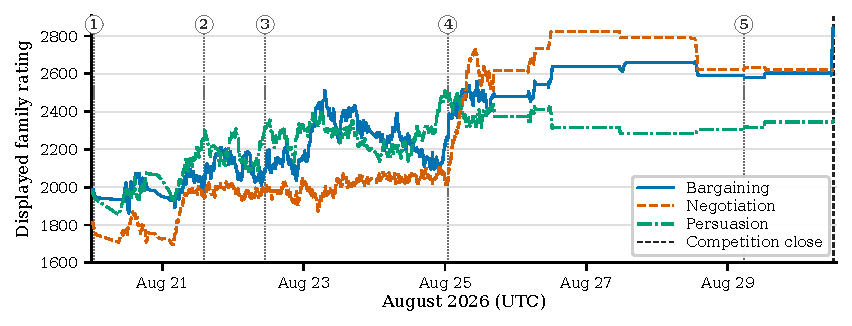
\includegraphics[width=\linewidth]{figures/fig_agent5_lifecycle.pdf}
  \caption{Focal-agent displayed ratings in 1,348 authenticated per-family API
  polls retained in the frozen dataset, from the first poll, after 3,545
  cumulative family games, through the first settled poll after close. Lines
  connect polls. Verified runtime boundaries are: (1) family-winner assembly;
  (2) bargaining stonewall rollback; (3) measurement reset after the
  persuasion backload test; (4) deterministic negotiation dispatcher
  activation; (5) final persuasion overlay and audit boundary. The close line
  marks competition end. None is an isolated treatment effect.}
  \label{fig:lifecycle}
\end{figure}

\section{Agent Behavior Analysis}
\label{sec:behavior}

We use two complementary denominators. The lifecycle census reads every 46,316
canonical local assignment record from August 19 to 30, spanning 512,456 nested
own actions. It describes an evolving policy, not one treatment. We did not
freeze a complete row-level official lifetime history. Because the retained
close snapshot is aggregate, the artifact cannot join all 46,316 local
assignments to the 46,564 official rated games. Table~\ref{tab:behavior}(a)
reports both without calling one coverage of the other. The final audit
censuses August 29 05:27--12:48 UTC and August 30
11:08--11:59 UTC; the agent was banked between them. The closing run contained
152 bargaining, 30 persuasion, and no negotiation assignments.

\begin{table}[H]
\centering
\scriptsize
\caption{Lifecycle and final-policy behavior. Local terminal failures are
timeouts or invalid termination. Official $\Delta R$ is the dashboard's
displayed per-game change; brackets are descriptive 95\% game-bootstrap
intervals for the mean.}
\label{tab:behavior}
\setlength{\tabcolsep}{2.6pt}
\renewcommand{\arraystretch}{0.96}
\begin{tabularx}{\linewidth}{@{}lrrYl@{}}
\toprule
\multicolumn{5}{@{}l}{\textit{(a) Entire local lifecycle and official endpoint}} \\
Family & Local games & Actions & Local outcomes/status & Official rating/games \\
\midrule
Bargaining & 15,539 & 96,756 & 15,483 agreements; 6 completed no-deals; 49 timeouts; 1 active & 2804.82/15,639 \\
Negotiation & 15,354 & 108,984 & 7,516 agreements; 5,591 no-deals; 2,177 walks; 67 timeouts; 3 active & 2620.36/15,415 \\
Persuasion & 15,423 & 306,716 & 15,306 completed; 105 timeouts; 1 invalid; 11 active & 2344.87/15,510 \\
\bottomrule
\end{tabularx}

\vspace{2pt}
\begin{tabularx}{\linewidth}{@{}lrrYl@{}}
\toprule
\multicolumn{5}{@{}l}{\textit{(b) Authenticated final-policy audit}} \\
Family & Rated/all & Zero/rated & Returned behavior and outcomes & Mean $\Delta R$ [95\%] \\
\midrule
Bargaining & 171/171 & 0/171 & 503 offers, 414 rejects, 84 accepts; 171 agreements & $1.26\ [.59,1.92]$ \\
Negotiation & 19/19 & 6/19 & 10 offers, 171 rejects/counters, 7 accepts, 2 own walks; 13 agreements & $-.05\ [-2.17,2.05]$ \\
Persuasion & 54/55 & 12/54 & buyer BUY/PASS 456/201; seller positive/negative 316/124; 1 timeout & $.76\ [-.31,1.81]$ \\
\bottomrule
\end{tabularx}
\end{table}

Negotiation also has an intermediate mechanism census beyond the small final
receipt window. From activation of the deterministic dispatcher on August 25,
2,499 local assignments produced 18,033 own actions. The current-seller
fallback owned 866 games and 9,795 actions, first-principles cells 519 and 948,
observed-leader buyer paths 1,095 and 7,271, and the standardized one-round
seller owner 19 and 19. A configured hidden cap-10 terminal-inference branch
selected no focal-agent action. These counts establish which rules owned
recorded behavior, not whether an owner improved rating.

The bounded final audit joins the 245 local games to the same 245 authenticated
replays, including 244 rated outcomes and one timeout. Protocol and role
attribution identified 2,288 focal moves, and every normalized local returned
action matched a valid replay move. The behavior largely matched design:
bargaining always reached agreement, negotiation retained both walking and
trading, and persuasion used both messages and both buyer actions. Yet agreement
was not itself success. Six of 19 negotiation games returned zero, and its mean
official change was near zero despite a 68\% agreement rate. Role means also
varied: bargaining Alice/Bob changes were 1.86/.61, negotiation seller/buyer
1.09/$-1.32$, and persuasion seller/buyer 1.29/.39.

An earlier authenticated 85-game negotiation snapshot sharpened this point:
44 games had negative displayed changes, including 21 agreements. One visible
one-round buyer earned 3,000 yet lost 6.1 rating points, while a hidden
one-round buyer earned 300,000 yet lost 8.1. Positive payoff and agreement were
therefore not reliable substitutes for the competition objective.

Alignment assurance combined a frozen source revision and overlay, gate
reachability tests, local state-plan-action records, terminal outcomes, and
authenticated replay receipt, following the general principle that agent
behavior requires execution-level observability \citep{seyedghorban2026observability,
zhang2025agentracer}. It was not exhaustive owner conformance:
\texttt{plan.component} exists for only 220 of 2,288 final actions and
\texttt{gates\_fired} for 1,207. We can verify what action left the local policy
and appeared in replay, but not reconstruct a selected owner for every turn.

\section{Results, failures, and lessons}
\label{sec:competition}

The account led by the focal agent finished second in the agent track and third
combined at 2590.02. Figure~\ref{fig:lifecycle} and Table~\ref{tab:behavior}
show that this endpoint was produced by adaptation across all families, not by
a monotone climb or a bargaining-only policy. Using first-own-action and
half-open phases ending August 22 10:54:50, August 24 20:05:52, and August 29
05:27:36 UTC, B/N/P assignments were 5,983/5,972/5,967 in rapid search,
6,322/6,335/6,321 in measurement, and 3,063/3,028/3,080 in deterministic
assembly. Each development phase exposed all three families substantially.

Opponent observation influenced the search but was never treated as proof.
Three then-leading negotiation profiles opened at roughly .92 to 1.05 of
visible surplus while our opening was about .681. This motivated a .95
open-claim challenger and later observed-leader buyer paths. Field drift and
agreement-conditioned samples made direct imitation unsafe, so the broad clone
was assigned by game hash and judged on all assignments. The observed
correlation explains why the strategy was tested; the stopped experiment
explains why it was not promoted wholesale.

Negative results changed the policy. Bargaining stonewall and economic stall
were removed after live divergence and exploit tests. A promising high-share
delay rule was found unreachable; under the later stack, waiting beat immediate
acceptance in all 14 joined triggers by 21.77 pot points on average. In
negotiation, a randomized 91-game leader clone had a positive point estimate
but an interval crossing zero, 6.14 percentage points more no-deals, and a
negative focal-agent stratum, so it was stopped. A later score-floor challenger
closed only 7 of 27 resolved fires and was rolled back. In persuasion,
LLM-generated wording converted at 46.3\% versus 55.3\% for templates, and a
randomized backload policy lost by .391 raw-percentile points in its strict
profitable cells. Both were removed.

Failures remained at close. In one buyer game, four warnings escaped the final
persuasion veto; the agent bought all four products and each was LOW. After
three passed positive recommendations, only 8 of 664 observed targeted LOW
seller recommendations converted. The final credibility reset was copied
before its source experiment reached its precommitted efficacy read. Finally,
the clearest same-overlay seesaw retained every family: across 79 August 27
games, bargaining gained 21.03 rating points while negotiation lost 33.78 and
persuasion lost 29.42. Overall fell from about 2592.11 to 2578.05. These are
descriptive diagnostics in a nonstationary field, not component effects.

\paragraph{Reproducibility and conclusion.}
Frozen receipts preserve source, overlay, aggregates, rating snapshots, final
replays, and mathematical checks. We plan to release sanitized
production-equivalent source and verifiers; private replays await data-use
approval.

The second-place result supports the competitiveness of measured revision
across all three families. Game theory supplied local owners, rank awareness
changed acceptable risks, and action auditing separated intended from returned
behavior. No single owner has causal credit for the placement.

\clearpage
\bibliographystyle{plainnat}
\bibliography{references}

\iftechnicalappendix
\clearpage
\appendix
\section{Formal objective and observability}
\label{app:objective}

This supplement separates mathematical consequences of the scoring rule from
assumptions about the live field. The distinction matters because an equation
can prove what a policy guarantees without proving that opponents will respond
as the policy hopes.

\subsection{Game and score notation}

A game has public configuration $c\in\mathcal C$, role $r\in\mathcal R$,
public history $H_t$, own type $\theta_i$, opponent type $\theta_{-i}$, action
$A_t$, terminal payoff $Y$, and opponent strength $s_o$. Player $i$ acts on
$I_{i,t}=(c,r,H_t,\theta_i)$; its own type is observed, while
$\theta_{-i}$ may remain hidden. The platform maps $Y$ to a raw within-cell
percentile $q=Q_{c,r,\tau}(Y)$ using the reference pool available at time
$\tau$, applies an undocumented cell-, opponent-strength-, and
time-specific adjustment $\widetilde q=h_{c,r,s_o,\tau}(q)$, abbreviated $h(q)$
when those inputs are fixed, and then applies Eq.~\eqref{eq:rating}. The public
documentation specifies the same-configuration, same-role comparison and the
normal completed-game rating update, but does not specify how ties are handled
\citep{gleecompetition2026}. Because the rules page is mutable, the version
accessed on 2026-08-30 is preserved in \path{docs/reference/glee-docs.md}.

For exposition, define the exact-equality midrank of a fixed reference multiset
$D=\{z_1,\ldots,z_n\}$ by
\begin{equation}
q_D(y)=\frac{1}{n}\sum_{i=1}^n
\left[\mathbf 1\{z_i<y\}+\frac12\mathbf 1\{z_i=y\}\right].
\label{eq:midrank}
\end{equation}
If $Z$ is uniformly sampled from $D$, then
$q_D(y)=\Prb(Z<y)+\tfrac12\Prb(Z=y)$, the usual probability-of-superiority
interpretation behind rank statistics \citep{mann1947test}. The local code uses
the same convention with a $10^{-9}$ numerical tolerance for equality, so
Eq.~\eqref{eq:midrank} is its mathematical idealization. Neither convention
should be stated as the official tie rule without organizer confirmation.

\begin{proposition}[Midrank jump]
For $y_1<y_2$, the local diagnostic rank gain is
\begin{equation}
q_D(y_2)-q_D(y_1)=\frac{1}{n}\left(
\#\{i:y_1<z_i<y_2\}+\frac12\#\{i:z_i=y_1\}
+\frac12\#\{i:z_i=y_2\}\right).
\end{equation}
\end{proposition}
\begin{proof}
Expand Eq.~\eqref{eq:midrank} at $y_2$ and $y_1$. Observations strictly below
$y_1$ cancel. An observation at $y_1$ contributes $1$ to the first rank and
$1/2$ to the second, every interior observation contributes $1$, and an
observation at $y_2$ contributes $1/2$ only to the first rank.
\end{proof}

The proposition explains why a one-cent change can cross a large atom and have
more rank value than a much larger monetary change elsewhere. It also shows
why pooling the wrong cells changes the optimization problem.

\begin{proposition}[Rating equivalence]
Assume $R$, $\eta>0$, and the opponent adjustment are fixed for the decision,
and that the rating clamp is inactive. For any two actions $a$ and $b$,
\[
\E[\Delta R\mid a]\geq \E[\Delta R\mid b]
\quad\Longleftrightarrow\quad
\E[\widetilde q\mid a]\geq \E[\widetilde q\mid b].
\]
\end{proposition}
\begin{proof}
Substituting Eq.~\eqref{eq:rating} gives
$\E[\Delta R\mid a]=\eta\{8000\E[\widetilde q\mid a]-2000-R\}$.
All terms other than $\E[\widetilde q\mid a]$ are fixed, and the remaining
coefficient is positive.
\end{proof}

After $g$ games in a family, the ranked public display is
\begin{equation}
R_g^{\mathrm{disp}}=1000+\frac{g}{g+30}
\left(R_g^{\mathrm{raw}}-1000\right).
\end{equation}
At fixed $g$, this positive affine transform preserves the within-game ordering.
The official rules state that the mature update rate is $\eta=.002$
\citep{gleecompetition2026}. Conditional on no penalty or clamp, a final block
of $n$ games therefore receives total raw-rating weight
$1-(1-.002)^n$. Across the two final-profile windows, the 171 bargaining, 19
negotiation, and 54 rated persuasion games received 28.99\%, 3.73\%, and
10.25\% total raw-rating weight. The closing window alone contributed 152
bargaining games and 29 rated persuasion games, or 26.24\% and 5.64\% total
weight. These blocks matter to the endpoint, but their unrandomized exposure in
a moving field does not cleanly evaluate the configured policy.
Eq.~\eqref{eq:rating} does not cover abandonment, which receives a direct fifth
percentile assignment, games dropped because no move was made, an opponent's
voided copy, daily activity penalties, or hourly decay. A binding clamp, a
changing reference pool or opponent model, and comparisons across current
ratings or game counts need not preserve the simple ordering. The proposition
is a one-step decision result for a normally completed, nonabandoned game, not a
theorem about final leaderboard position.

\begin{proposition}[Dominance boundary under rank scoring]
For a fixed nondecreasing raw-rank map $Q$, if
$Y_A\geq Y_B$ almost surely, then
$\E[Q(Y_A)]\geq\E[Q(Y_B)]$. A larger expected payoff alone does not imply this
ordering.
\end{proposition}
\begin{proof}
Monotonicity gives $Q(Y_A)\geq Q(Y_B)$ almost surely, so taking expectations
preserves the inequality. The next proposition supplies a counterexample when
only the payoff means are ordered.
\end{proof}

\begin{proposition}[Expected payoff can reverse expected raw rank]
There exist a monotone percentile map $Q$ and actions $A,B$ such that
$\E[Y_B]>\E[Y_A]$ but $\E[Q(Y_B)]<\E[Q(Y_A)]$.
\end{proposition}
\begin{proof}
Use the exact empirical midrank in Eq.~\eqref{eq:midrank} with reference
multiset $D=\{5\}$. Action $A$ pays $10$ surely, while action $B$ pays $0$ or
$21$, each with probability $1/2$. Then
$\E[Y_A]=10<10.5=\E[Y_B]$. However,
$\E[q_D(Y_A)]=1$, while
$\E[q_D(Y_B)]=\{q_D(0)+q_D(21)\}/2=1/2$. Figure~\ref{fig:rank} plots this
finite empirical construction.
\end{proof}

This construction does not by itself order $\E[h(Q(Y))]$ for an arbitrary
nonlinear opponent adjustment. It carries through to expected adjusted rank,
and hence to one-step rating under the preceding proposition, when
$h(q)=a+bq$ with $b>0$, or whenever the fixed adjustment otherwise
preserves the two expectation orderings. The public formula is unavailable, so
the main paper keeps the raw-rank reversal and rating equivalence distinct.

\begin{figure}[h]
  \centering
  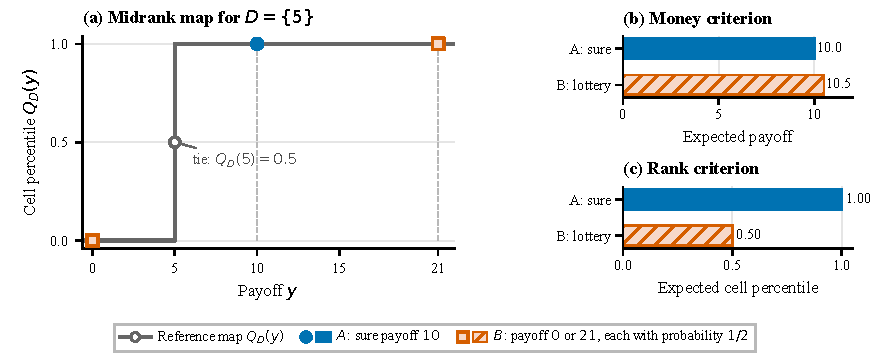
\includegraphics[width=0.96\linewidth]{figures/fig_rank_objective.pdf}
  \caption{Finite empirical payoff-rank reversal, not an estimated GLEE cell.
  Against the reference multiset $D=\{5\}$, action $A$ returns $10$ surely,
  while action $B$ returns $0$ or $21$ with equal probability. Therefore
  $\mathbb{E}[Y_B]=10.5>\mathbb{E}[Y_A]=10$, but
  $\mathbb{E}[Q_D(Y_B)]=0.5<\mathbb{E}[Q_D(Y_A)]=1$.}
  \label{fig:rank}
\end{figure}

\begin{proposition}[Terminal proposal value]
Suppose a proposal $x$ is accepted with probability $A(x)$, yields payoff
$u(x)$ if accepted, and yields zero if rejected. For a fixed raw percentile map
$Q$,
\[
\E[Q(Y)\mid x]=Q(0)+A(x)\{Q(u(x))-Q(0)\}.
\]
\end{proposition}
\begin{proof}
Condition on acceptance and rejection, then collect the two terms.
\end{proof}

The baseline $Q(0)$ is not generally zero. Under local midranks, if every
reference payoff in the cell is zero, then $q_D(0)=1/2$. This is a sufficient
condition for a zero to be locally neutral. Strategic infeasibility alone is
not sufficient because irrational trades, invalid outcomes, or a mixed
reference population can place nonzero mass elsewhere.

\subsection{Hidden-type non-identification}

Let the same information state $I_{i,t}$ arise under two observationally
equivalent opponent types $\theta_{-i}^{(1)}$ and $\theta_{-i}^{(2)}$. Any
deterministic policy $\pi_i(I_{i,t})$ must take the same action under both. If
one type pair admits gains from trade and the other does not, no such policy can
condition on true feasibility before a revealing action occurs. A prior
over types can support a Bayesian action, but the prior is a modeling
assumption when hidden opponent values are never revealed. In particular, the
observed competition logs do not nonparametrically identify the hidden joint
type frequencies or the response to an offer that was never sent.

\section{Audited submitted policy specification}
\label{app:policy}

Shapira et al. organize GLEE by game family, horizon, information structure,
and communication form \citep{shapira2024glee}. We use the same vocabulary but
do not equate the live competition grid with the benchmark paper's experimental
grid. Version 3 of the benchmark paper reports 1,320 configurations: 384
bargaining, 576 negotiation, and 360 persuasion. The competition documentation
reports 960 total but no family decomposition. Our observed-server
reconstruction gives 384, 396, and 180 respectively, conditional on its
reconstructed negotiation support and long-living-only persuasion model. Those
family counts are our reconstruction, not an organizer-published fact. In
particular, the live state exposed no myopic-buyer flag, and the policy used the
full persuasion history. A publicly undisclosed long horizon is called
``infinite'' in the benchmark paper, but the agent treated it as long and
unknown rather than literally unbounded.

The launch record fixes source commit
\texttt{b54cb33ad9f4fe7da4c667262eee00ffaeac3ab6}. The complete recorded 81-key
overlay receipt, together with the separately hashed persuasion and
nonpersuasion dictionaries, is in
\path{paper/data/submitted_agent_bank_manifest.csv}.
The behavior-affecting values absent from that overlay were LLM mode off;
bargaining hidden-opponent discount $.90$ and undisclosed-horizon cap 99; and
negotiation assumed horizon 10, deal odds $.65$, and Boulware exponent $2.0$.
These values are recorded beside the overlay rather than silently treated as
flags. The following pseudocode
gives exact owner precedence, not a self-contained replacement for the full
action function. History state, fitted tables, parser details, and postguards
remain in the versioned source. The family sections below derive the policy
pieces needed to interpret those branches, and
\path{paper/analysis/verify_theory_code.py} checks selected outputs against the
implementation.
That verifier checks selected algebra and branch outputs. It does not verify
effective live flags, every routing path, process provenance, server receipt, or
the causal value of a policy.

\begin{center}
\fbox{\begin{minipage}{0.95\linewidth}
\small\ttfamily
BANKED-ACTION($g$):\\
\hspace*{1em}if family($g$) = bargaining:\\
\hspace*{2em}if silent-Bob-$T12$-$\delta_2{=}.95$ eligible:
  $a\leftarrow$ P2-FIXED-POLICY($g$)\\
\hspace*{2em}else: $a\leftarrow$ GENERIC-BARGAIN($g$), including eligible BOB-RANK-FLOOR\\
\hspace*{1em}else if family($g$) = negotiation:\\
\hspace*{2em}if one-round-seller eligible:
  $a\leftarrow$ FIRST-PRINCIPLES($g$)\\
\hspace*{2em}else if complete-$T10$-buyer eligible:
  $a\leftarrow$ FIRST-PRINCIPLES($g$)\\
\hspace*{2em}else if hidden-$T10$ terminal bound exists:
  $a\leftarrow$ BOUND-PLUS-CENT($g$)\\
\hspace*{2em}else if role($g$) = buyer:
  $a\leftarrow$ LEADER-BUYER-PATH($g$)\\
\hspace*{2em}else:\\
\hspace*{3em}$a\leftarrow$ GENERIC-SELLER($g$)\\
\hspace*{3em}if seller-message cell: overwrite only $a$.message from table\\
\hspace*{1em}else if family($g$) = persuasion and role($g$) = seller:\\
\hspace*{2em}$a\leftarrow$ SELLER-RULE(quality, prior EV, historical buy rate)\\
\hspace*{1em}else:\\
\hspace*{2em}$a\leftarrow$ BUYER-V2-POSTERIOR-MONEY-GATE($g$)\\
\hspace*{2em}$a\leftarrow$ TIGHT-CREDIBILITY-RESET-V1($g,a$)\\
\hspace*{2em}if explicit decline and $a=$ BUY: $a\leftarrow$ PASS\\
\hspace*{1em}return COERCE-POSTGUARD-OR-SAFE-FALLBACK($a,g$)
\end{minipage}}
\end{center}

\begin{table}[h]
\centering
\small
\caption{Policy ownership across the GLEE market dimensions. ``Either'' means
the owner did not require that dimension, not that the two conditions are
strategically equivalent.}
\label{tab:policy_ownership}
\begin{tabularx}{\linewidth}{@{}p{2.1cm}p{3.5cm}p{3.4cm}Y@{}}
\toprule
Family and role & Horizon, information, communication & Highest eligible owner & Returned behavior \\
\midrule
Bargaining, Bob & Disclosed $T=12$, own $\delta=.95$, no messages; either information state & Narrow self-commitment rule & Bob-share ladder $.61,.68,.74,.82,.91$, then $M-.01$; common discounted terminal floor on decisions. \\
Bargaining, either & Every other supported cell & Generic planner & Finite recursion when $T$ is disclosed; otherwise a reconstructed 99-round cap plus an inflation-aware concession clock capped at 60, followed by continuation and empirical floors. Eligible Bob offers add a local raw-rank floor. \\
Negotiation, seller & Disclosed $T=1$; complete or hidden; structured or linguistic & One-round structural owner & Ask visible buyer value minus one cent, or use the hidden support-grid ask. It emits no text even when text is allowed. \\
Negotiation, buyer & Complete, disclosed $T=10$ & Complete structural owner & Counter at seller value plus one cent; hold for $.994$ of visible surplus off terminal; accept positive terminal gain. \\
Negotiation, buyer & Hidden, disclosed $T=10$, terminal offer & Conditional support-bound owner & Retain seller asks strictly below $b$; choose the greatest support cost strictly below $b$ and no larger than their minimum, then bid one cent above it. \\
Negotiation, either & Remaining buyer or seller states & Buyer path or seller fallback & Fixed observed-leader buyer paths; Boulware, continuation, stall, and endgame seller bundle. Supported seller cells may receive a message-only rewrite. \\
Persuasion, seller & Known or hidden buyer value; binary or text & Seller rule & Recommend HIGH; handle LOW by prior expected value when buyer value is known, otherwise by historical buy rate. Emit literal yes/no tokens. \\
Persuasion, buyer & All supported histories and message modes & Posterior, reset, veto & Posterior monetary gate, tight credibility reset, then a final recognized-decline BUY-to-PASS veto. \\
\bottomrule
\end{tabularx}
\end{table}

\begin{table}[h]
\centering
\small
\caption{Objective and evidence class of each retained owner group. The rank
objective governed evaluation; two retained subcomponents optimized local
raw-rank models directly.}
\label{tab:owner_objectives}
\begin{tabularx}{\linewidth}{@{}p{3.0cm}p{3.8cm}p{4.0cm}Y@{}}
\toprule
Owner group & Action objective or invariant & Warrant & Claim boundary \\
\midrule
Generic bargaining & Discounted monetary continuation, then empirical own- and opponent-share floors; eligible Bob asks add a local raw-rank floor & Finite backward induction plus fitted acceptance, coarsened CDF, and refusal-continuation heuristics & The Bob search is a coarsened local raw-rank proxy, not the official adjusted scorer; the hidden 99-round cap and effective concession clock are reconstructed or heuristic. \\
Narrow silent bargaining & Fixed Bob-share ladder and discounted terminal floor & Internal policy discipline, reached-action audit, and selected closures & Neither observable commitment nor a causal field-effect estimate. \\
One-round hidden seller & Equal-weight seed-CDF average over latent buyer support, message modes, and scales & Exact checked-in seed CDFs and server support reconstruction & Second direct local-rank proxy; the pooled bank is not conditionally optimal in every visible cell or for the official opponent adjustment. \\
Complete negotiation owners & Maximize own monetary surplus subject to a strictly positive modeled opponent gain & Visible gains from trade and selected terminal-response audit & Acceptance is behavioral, not guaranteed; reached states are selected. \\
Hidden terminal buyer & Preserve positive own surplus using an offer-implied reservation bound & Seller individual rationality and discrete support & The premise can fail, and no rank optimum is claimed. \\
Buyer and seller fallbacks & Agreement and monetary continuation through leader paths or Boulware-style concession & Public trajectories and empirical heuristics & Retained for coverage; standalone value remains unidentified. \\
Persuasion seller & Sale count under a one-shot obedience guide and an adaptive buy-rate cutoff & Bayesian benchmark plus repeated-history heuristic & GLEE is repeated noncommitted cheap talk, not committed persuasion. \\
Persuasion buyer & Posterior expected money, followed by credibility and semantic safety guards & Regularized Bayesian-style model and returned-action audits & Not dynamically or rank optimal; veto effect remains unknown. \\
\bottomrule
\end{tabularx}
\end{table}

The policy is deterministic conditional on the full request, effective overlay
and runtime defaults, frozen model contents and cache state, and the parser,
coercion, and source versions. Every enumerated randomized A/B and probe flag
was zero at bank, so disabled game-ID hash arms did not change its actions. The
final action layer still matters. Owners in the structural negotiation path are exempt from generic
price rewrites, while generic complete-information seller openings are
rewritten to claim $.95$ of visible surplus and later asks are floored at
$.80$. Coercion repairs repairable candidates. A non-dictionary, unknown action
type, unrepairable \texttt{InvalidAction}, or price-guard failure uses the legal
family \texttt{safe\_action}. A dispatcher exception first coerces that safe
action and uses \texttt{\_last\_resort} only if this also fails. Thus the
planner's intermediate action is not always the returned action.

The bargaining ladder is deterministic internal policy discipline. It is not
an observable commitment device, since the eligible cell is silent, and it is
not a claimed equilibrium commitment.

Outside that preempting cell, the active generic Bob-offer subcomponent used a
direct local-rank objective. Let $a$ be Bob's share of the pot, $r$ the current
round, $d$ the opponent's latest demand, and
$\kappa(c)=(M,T^{\mathrm{field}},\mathbf 1\{T\text{ known}\},
\mathbf 1\{\text{complete information}\})$ the fitted CDF key for public
configuration $c$, where $T^{\mathrm{field}}$ is the transmitted maximum-round
field and may be absent. This key omits acting role, both discount factors, and
message mode, so its training CDF pools those dimensions. It also omits the
undocumented opponent-strength adjustment and the time-varying reference pool.
Writing $\widehat Q_{\kappa(c)}$ for this coarsened empirical midrank CDF, the
component evaluated
\begin{equation}
J(a)=\widehat P_{\mathrm{acc}}(1-a,r,\delta_{-i},d)
      \widehat Q_{\kappa(c)}(a\delta_i^{r-1})
 +\{1-\widehat P_{\mathrm{acc}}(1-a,r,\delta_{-i},d)\}
      \widehat V_{\mathrm{cont}}(r,\delta_i).
\label{eq:bob_rank_search}
\end{equation}
The search starts at the greater of the generic baseline ask and the best share
the opponent has already offered Bob, advances in $.01$ share increments, and
is globally restricted to $[.20,.95]$. Ties select the larger ask. It changes
the returned target only when the best $J(a)$ exceeds
$\widehat V_{\mathrm{cont}}$ by more than $.005$, and only as an upward floor:
the model's downward-concession recommendation was not deployed. The fitted
logistic acceptance model, coarsened CDFs, and refusal-continuation table are in
\path{models/barg_bob_offer_v1.json}. An absent $\kappa(c)$ bucket uses the
fully pooled CDF. Only the absence of a usable loaded or cached model leaves the
baseline unchanged. This is the first of the two direct local-rank components;
it does not compute GLEE's undisclosed opponent adjustment.

\FloatBarrier
\section{Bargaining derivations}
\label{app:bargaining}

Consider a divisible unit pie, alternating proposals, zero disagreement payoff,
complete information and common knowledge of a finite number $k$ of proposal
opportunities and discount factors $\delta_i,\delta_j\in(0,1]$, and acceptance
of offers that make the responder indifferent. Let $f_i(k)$ be player $i$'s
share when $i$ proposes with $k$ opportunities remaining. These assumptions do
not describe GLEE cells where the opponent discount or true horizon is hidden;
there the recursion is a planning benchmark rather than a Bayesian equilibrium.

\begin{proposition}[Finite-horizon recursion]
The subgame-perfect proposer share satisfies
\begin{equation}
f_i(1)=1,\qquad f_i(k)=1-\delta_j f_j(k-1).
\label{eq:finite_recursion}
\end{equation}
If a stationary limit exists and $\delta_i\delta_j<1$, then
\begin{equation}
f_i^*=\frac{1-\delta_j}{1-\delta_i\delta_j},\qquad
f_j^*=\frac{1-\delta_i}{1-\delta_i\delta_j}.
\end{equation}
\end{proposition}
\begin{proof}
With one opportunity left, the proposer can retain the entire pie while giving
the responder its rejection value of zero. With $k>1$, rejection makes player
$j$ the next proposer, where $j$ receives $f_j(k-1)$ one period later. Player
$i$ therefore offers $\delta_j f_j(k-1)$ and retains the remainder, proving the
recursion by backward induction. At a stationary limit,
$f_i^*=1-\delta_j f_j^*$ and $f_j^*=1-\delta_i f_i^*$. Substitution and division
by $1-\delta_i\delta_j$ give the result.
\end{proof}

When $\delta_i=\delta_j=1$, the stationary equations do not select a unique
split. The helper returns an equal split only when called with no numerical
horizon or more than 200 opportunities. The deployed generic planner does not
use that branch for the public no-limit state. It substitutes a 99-opportunity
recursion horizon and, in the dated submitted-agent profile, a separate 60-round cap for
concession pacing. Its resulting parity and artificial terminal boundary are
heuristics, not equilibrium consequences of a genuinely unlimited game. Known
finite horizons retain the backward-recursion parity. The finite result follows
under the stated terminal rule; the stationary formula is the Rubinstein benchmark
\citep{rubinstein1982}. The connection between
axiomatic Nash bargaining and strategic alternating-offer models is discussed
by \citet{binmore1986nash}.

\begin{proposition}[Patient-responder parity]
If responder $j$ has $\delta_j=1$, then for every integer $m\geq0$,
\[
f_i(2m+1)=\delta_i^m,\qquad f_i(2m)=0\quad(m\geq1).
\]
\end{proposition}
\begin{proof}
The base cases are $f_i(1)=1$ and
$f_i(2)=1-f_j(1)=0$. Assume the claim through $2m$. The alternating recursion
gives $f_j(2m)=1-\delta_i f_i(2m-1)=1-\delta_i^m$, so
$f_i(2m+1)=1-f_j(2m)=\delta_i^m$. It then gives
$f_j(2m+1)=1-\delta_i f_i(2m)=1$, so
$f_i(2m+2)=1-f_j(2m+1)=0$.
\end{proof}

\subsection{Continuation values and safe decisions}

With pie size $M$ and $k\geq2$, a responder $i$ who rejects
becomes proposer next period and has equilibrium continuation
$\delta_i f_i(k-1)M$. A current proposer $i$ whose offer is refused becomes
the next responder and has continuation
$\delta_i[1-f_j(k-1)]M$. These are model-based continuation values. The live
policy additionally uses a fairness floor and a trend estimate from observed
concessions, so its final aspiration is a heuristic blend rather than an
equilibrium theorem.

\subsection{Exact generic bargaining order at the submitted bank}

This subsection excludes the preempting silent Bob owner. Let $M$ be the pie,
$r$ the public round, $\delta_i$ our discount, and $\delta_j$ the disclosed
opponent discount or $.90$ when hidden. The planner sets $k=T-r+1$, where $T$
is the disclosed cap or the reconstructed value $99$ when the horizon is
withheld. Since $k\leq99$, production uses Eq.~\eqref{eq:finite_recursion}, not
the stationary-limit branch. With full recursion weight one, the aspiration
before later transforms is
\begin{equation}
a_0=\min\{M,\max[f_i(k)M,\ .57M,\ C_i^{\rm ref}]\},\qquad
C_i^{\rm ref}=\begin{cases}
0,&k=1,\\
\delta_i[1-f_j(k-1)]M,&k>1.
\end{cases}
\label{eq:generic_barg_aspiration}
\end{equation}
Thus $.57$ is an intermediate floor, not a returned-offer invariant.

Only when the horizon is hidden, the pacing clock is
\begin{equation}
H_i=\begin{cases}
\max\{4,\min[\lceil\log(.05)/\log\delta_i\rceil,60]\},
   &0<\delta_i<1,\\
60,&\delta_i\geq1.
\end{cases}
\label{eq:effective_barg_horizon}
\end{equation}
It equals $14,29,59,60$ on the supported grid
$\delta_i=.8,.9,.95,1$. Therefore $60$ is a cap, not a common clock. With
$e=\min\{1,\max[0,(r-1)/H_i]\}$ and $L$ the larger of realistic continuation
and the best recorded opponent offer to the agent, capped at $M$, the target
becomes $L+(a_0-L)(1-e)^2$ when $a_0>L$.

Offer transforms then run in source order. At $k=1$ the planner first sets own
gain to $.75M$; at $k=2$ it applies
$\max\{C_i^{\rm ref},\min(a,.62M)\}$. It next enforces the submitted
opponent-share floor $.39$, capping own gain at $.61M$. Consequently the
ordinary generic terminal proposal is $.61M$ before numeric coercion. On Bob
offer turns with $k>2$, the local-rank transform may then raise, but never
lower, this baseline. Its lower bound is the larger of the baseline and Bob's
best recorded incoming share. It searches $.01$ increments within $[.20,.95]$,
breaks ties upward, and acts only when expected local percentile exceeds fitted
refusal continuation by more than $.005$. The configured high-share guard is
unreachable because its required deterministic no-regression parent is off.

On a decision turn, $k\leq1$ accepts exactly when incoming gain is strictly
positive. Otherwise the threshold begins at $.98R_i$, where $R_i$ is realistic
continuation: the equilibrium continuation $\delta_if_i(k-1)M$, except that
the $\delta_j=1,k>2$ corner uses $.57\delta_iM$ as a ceiling, and at least two
opponent offers can lower that ceiling through a first-to-last concession
projection over at most five future steps. For $k>2$, the bank raises the
threshold to at least $F_iM$, where
\begin{equation}
F_i=\begin{cases}
\min\{.50,\delta_i(.05)/(1-\delta_i)\},&\delta_i<1,\\
.50,&\delta_i=1.
\end{cases}
\label{eq:generic_barg_accept_floor}
\end{equation}
Observed-gain replacement, stonewall release, economic-stall release,
opponent exploitation, and no-regression guards are off. If this threshold
still rejects a strictly positive offer in a hidden-horizon game at
$r\geq H_i$, the pacing fallback changes the decision to acceptance.

The bargaining message arm and LLM path are off. The dispatcher strips
diagnostics and coerces the planned action. For an integer pie, a generic offer
rounds the acting player's gain to a whole unit and computes the other gain as
the exact complement. A noninteger pie uses cent rounding with residual repair.
Decision aliases are normalized and forbidden or malformed messages removed.
An unknown or unrepairable action uses an even split on an offer or acceptance
on a decision. These are local post-coercion returns, not proof of server
receipt. At the $.8$ and $.9$ floor settings, ordinary floating-point
evaluation gives values just above $.20$ and $.45$; the exact-equality repair
was off at bank, so a wire-exact boundary offer could be rejected by a few
units in the last place.

\begin{proposition}[Terminal positive acceptance]
At a genuinely terminal decision, accepting a strictly positive monetary
payoff strictly dominates rejection payoff zero. Under any nondecreasing
percentile map, it weakly dominates in raw rank.
\end{proposition}
\begin{proof}
The monetary claim follows from $y>0$. Monotonicity gives $Q(y)\geq Q(0)$.
\end{proof}

\begin{proposition}[Limited discounted guard]
Let $o$ be a current offer to player $i$. Consider only the continuation action
that sends a counter giving player $i$ payoff $c$ if the opponent accepts it
exactly one period later.
If $o\geq\delta_i c$, accepting now weakly dominates that continuation in
discounted money.
\end{proposition}
\begin{proof}
Acceptance pays $o$ now. The stipulated continuation pays $c$ one period later,
with present value $\delta_i c$.
\end{proof}

The qualification is essential. The guard does not dominate a policy that
chooses a different counter, receives a new opponent offer, or reaches a better
agreement several rounds later. A retrospectively selected corpus contained
49/49 favorable comparisons for $\delta<1$, with mean gain $0.03326$ of the pie
and nominal game-bootstrap interval $[0.02722,0.03930]$. At the patient boundary
$\delta=1$, 16 decisions averaged $-0.0505$. The interval is descriptive
conditional on the selected rule and corpus. The candidate excluded the patient
boundary, but was later retired; the broad guard was off at the submitted-agent bank.

\subsection{Heuristics and their status}

\begin{table}[h]
\centering
\small
\caption{Bargaining rules separated by what they actually guarantee.}
\label{tab:barg_heuristics}
\begin{tabularx}{\linewidth}{@{}p{3.1cm}p{5.0cm}Y@{}}
\toprule
Rule & Exact property & What remains empirical \\
\midrule
Finite recursion & Eq.~\eqref{eq:finite_recursion} under the alternating-offer assumptions and a real finite horizon. & Opponents need not play the equilibrium response; the no-limit state uses a reconstructed cap and synthetic effective clock. \\
Planner aspiration floor & Before later offer transforms, aspiration is at least the configured own-share floor and computed refusal continuation. & Endgame caps, opponent floors, and seat-specific owners can replace or lower the transmitted offer. \\
Observed concession projection & After at least two opponent offers, nonpositive trend uses the latest gain one period later; positive trend searches up to five steps. Both are capped by the model or field ceiling. & With fewer than two offers the ceiling stands. The broad observed-gain deployment measured negative on three seeds: $-0.0012,-0.0013,-0.0006$. \\
One-decision-period gain threshold & For $0<\delta<1$, if the next accepted payoff is exactly $s+G$ one discount period later, waiting is preferred to $s$ when $s<\delta G/(1-\delta)$. At $\delta=1$, it is preferred whenever $G>0$. & The mapping from public rounds to one discount period is a heuristic. The assumed $G=0.05$ was not reached in 895 measured continuations; median realized gain was $0.0012$. \\
Fixed P2 policy & Odd-round decisions check a common discounted floor. The bank-enabled silent policy sends a fixed $.61/.68/.74/.82/.91$ Bob-share ladder and gives Alice one cent on round 12. & Bank-enabled only in Bob/P2, messages-off, disclosed-12-round, $\delta_2=.95$; internal discipline, not an observable commitment device or a guarantee of agreement or optimality. \\
Broad discounted guard & If active, the limited dominance result above applies in its exact scope. & Retrospective candidate; retired and off at the dated bank. \\
\bottomrule
\end{tabularx}
\end{table}

\section{Negotiation derivations}
\label{app:negotiation}

Let a seller value the item at $s$, a buyer value it at $b$, and a transaction
occur at price $p$. Seller payoff is $p-s$ and buyer payoff is $b-p$.

\begin{proposition}[Strict gains from trade]
A price giving both players strictly positive payoff exists if and only if
$b>s$. The set of such prices is $(s,b)$.
\end{proposition}
\begin{proof}
Both payoffs are positive exactly when $p>s$ and $p<b$, which is possible
exactly when $s<b$.
\end{proof}

The checked-in reconstructed generator contains six complete-information cells,
all feasible, and 16 hidden type pairs, of which six satisfy $b>s$. Treating
seller and buyer types as independent and uniform assigns the hidden feasible
pairs probability $6/16=37.5\%$. If the combined 22-point value-information
axis is also sampled uniformly, 10/22, or 45.45\%, of its points are infeasible.
The support counts are structural conditional on the reconstruction; both
probability statements additionally require weighting assumptions the logs do
not identify. Neither result is an application of the
Myerson--Satterthwaite impossibility theorem. That theorem concerns full
efficiency under independently drawn, overlapping private-value support,
incentive compatibility, individual rationality, and budget balance
\citep{myerson1983bilateral}.

The hidden one-round seller used an explicit four-point table. Let
$\mathcal V=\{.8,1.0,1.2,1.5\}$ be the normalized value support,
$\mathcal B=\{100,10^4,10^6\}$ the three monetary bases, and
$\mathcal M=\{0,1\}$ the no-message and message modes. For normalized seller
cost $s\in\mathcal V$, candidate target $x>s$, and base $B$, the transmitted
ask is $p_x(B)=xB-.01$. For each latent buyer value $vB$, define the seller
payoff under threshold acceptance as
\begin{equation}
Y_{s,v,B}(x)=\mathbf 1\{vB>p_x(B)\}\{p_x(B)-sB\}.
\end{equation}
The exact seed CDF changes with the latent value pair. The bank therefore used
the pooled ex ante objective
\begin{equation}
\overline J_s(x)=\frac{1}{24}
\sum_{B\in\mathcal B}\sum_{m\in\mathcal M}\sum_{v\in\mathcal V}
Q^{\mathrm{seed}}_{c(1,\mathrm{hidden},m,B,s,v),\mathrm{seller}}
\!\left(Y_{s,v,B}(x)\right),
\label{eq:hidden_seller_seed_objective}
\end{equation}
which weights the four latent buyer values, two message modes, and three scales
equally. It does not hold the latent value pair, message mode, or scale fixed.
The checked-in exact seed CDF gives
\begin{center}
\small
\begin{tabular}{@{}lll@{}}
\toprule
$s$ & Candidate $x:\overline J_s(x)$ & Bank target \\
\midrule
$.8$ & $1.0:.271781,\ 1.2:.377128,\ 1.5:.359457$ & $1.2$ \\
$1.0$ & $1.2:.282183,\ 1.5:.250627$ & $1.2$ \\
$1.2$ & $1.5:.246189$ & $1.5$ \\
$1.5$ & no supported $x>s$ & $2.0$ \\
\bottomrule
\end{tabular}
\end{center}
Thus costs $.8B,1.0B,1.2B,1.5B$ produced asks
$1.2B-.01,1.2B-.01,1.5B-.01,2.0B$, respectively. At the top cost no supported
buyer value exceeds cost, so $2B$ is a deterministic dead-cell convention, not
a unique maximizer. In some fixed message-scale cells the $.8B$ argmax differs
from $1.2B-.01$; the hard-coded bank is an optimizer only for the declared
24-cell average. Threshold acceptance and equal weights are construction
assumptions, not identified live response or exposure frequencies. The result
is a frozen seed-rank proxy, not an optimizer for the undocumented opponent
adjustment or later field.

\begin{proposition}[Conditional bounds from offers]
Assume every buyer proposal would give the buyer nonnegative payoff if accepted,
and every seller proposal would give the seller nonnegative payoff if accepted.
Then every observed buyer bid satisfies $p_b\leq b$, and every observed seller
ask satisfies $p_s\geq s$. If the relevant observed set is nonempty, the maximum
buyer bid is a lower bound on $b$, and the minimum seller ask is an upper bound
on $s$.
\end{proposition}
\begin{proof}
Nonnegative buyer payoff gives $b-p_b\geq0$. Nonnegative seller payoff gives
$p_s-s\geq0$. Taking extrema preserves the inequalities.
\end{proof}

The assumption is not cosmetic. The corpus includes loss-making offers and a
small number of agreements outside the rational support. The policy therefore
treats these bounds as conditional evidence, not revealed truth.

The submitted hidden terminal buyer applies the bound only after retaining
seller asks $A_s$ strictly below its own value $b$. When $A_s$ is nonempty, it
computes
\begin{equation}
\hat s=\max\{s'\in\mathcal S:s'<b,\ s'\leq\min A_s\}
\end{equation}
when that set is nonempty, then bids $\hat s+.01$. Calling $\min A_s$ a cost
upper bound relies exactly on the seller individual-rationality premise above.

\subsection{Exact banked negotiation order}

The whole-policy order differs from the order inside the generic fallback.
First, a promoted one-round seller owner handles disclosed $T=1$ offer states,
asking $b-.01$ when values are visible and using the frozen support-grid ask
when they are hidden. The submitted direct router then owns the designed
one-round seller and complete-information $T=10$ buyer cells. Next comes the
unflagged hidden $T=10$ terminal-bound inference above, followed by the
observed-leader buyer tables. All supported buyer states therefore return
before the generic planner. The generic path is effectively the remaining
seller policy on the official grid. Its price-bearing output may receive the
seller message-only overlay, then schema coercion and numeric postguards.
Direct structural, inferred, and buyer-table wires bypass those generic numeric
postguards. Successor-policy seller rewrites were not part of the submitted
bank.

After the generic planner has constructed a target, its decision owner uses
the following source order:
\begin{enumerate}
  \item At a true disclosed terminal, accept exactly when the current price
  gives strictly positive own gain. Equality rejects, and this branch preempts
  every item below.
  \item In an uncapped deadgame state, walk only after elapsed fraction $.60$,
  an unprofitable current offer, and detected opponent stall.
  \item With a visible positive span and outside a true terminal, reject when
  own share is strictly below $.48$. Equality passes this veto.
  \item At an eligible real-cap final-proposer state, reject when current
  surplus is below the $.60$ option value.
  \item In hidden-value states, apply the learned acceptance table.
  \item Accept a profitable price within one percent of the returned stall
  price when the last three opponent offer records vary by at most one percent.
  \item Otherwise accept a strictly profitable offer when current surplus is
  at least
  \begin{equation}
  v_{\rm cont}=.65\left(1-\frac1R\right)\widehat u,
  \label{eq:nego_continuation}
  \end{equation}
  where $R$ is planned rounds left and $\widehat u$ is projected surplus.
  \item Otherwise reject and counter, using the more favorable of the incoming
  and target prices for the acting role.
\end{enumerate}
The final-option value in complete information is
$.60(1-.39)=.366$ of visible span and is shadowed by the earlier $.48$ veto.
It is also unreachable on the supported banked route because the relevant
$T=10$ buyer is direct-owned. The configured $.80$ ultimatum writer is likewise
shadowed on supported returned wires. These nonzero settings are not evidence
that the corresponding branch acted.

The active learned table has no ask map, so only its hidden acceptance rows
operate. In elapsed quartile
$q=\min\{\lfloor4e\rfloor,3\}$, its seller thresholds are
$(.4984083690,.4363183570,.0344636090,.2268590560)B$ and its buyer thresholds
are $(.1326067285,.3296081160,.0759175182,.1184233009)B$. Under the whole-policy
precedence, only hidden generic sellers normally reach these values.

The generic seller target itself runs through: assumed horizon 10 with a
separate real-cap marker; anchor $4s$; an observed buyer-bound floor; a
reservation with minimum margin $.02$, visible opponent share $.39$, and a
hidden $1.5B$ seller floor of $1.15s$; a power-2 Boulware path; the visible-ZOPA
clamp; terminal, stall, deadgame, posterior, and curve writers in source order;
the $.40$ outgoing-span invariant; then cent rounding. Rank-pricing and split
transforms were off. After the optional message-only overlay and coercion, the
final numeric postguard sets the first outgoing generic complete-information
seller price to exactly a $.95$ own-span claim and floors later prices at $.80$,
clamped inside the visible ZOPA. A first rejection counter counts as the first
outgoing price. Hidden sellers have no visible-span postguard, while direct
wires are exempt.

The deadgame target writer and the later walk decision are separate. The writer
requires the structurally dominated own draw, an opponent bound, and at least
four collected opponent offer records; it writes a positive-margin target. The
walk additionally requires the uncapped, stalled, late, currently unprofitable
state. The collected records include offers and counteroffers and deduplicate
only identical round-price pairs, so they are not necessarily four distinct
utterances.

\subsection{Retained empirical buyer table}

The remaining buyer path counts prior distinct own price utterances $k$ and
holds the final table entry after the sequence ends. With complete information,
let $Z=b-s$. A disclosed cap-10 game uses buyer-share sequence
$(.960,.898,.836,.774,.774)$ and an undisclosed horizon uses
$(.960,.898,.836,.774,.712)$, returning price $b-\rho_k Z$. A one-round
complete buyer uses the first cap-10 entry unless the structural terminal owner
preempts it. Off terminal it accepts a profitable seller ask no larger than the
price implied by the sequence's final share. At a true terminal receiver state
it accepts exactly when $b-p>0$.

For hidden information, write the buyer's own value as $mB$. The literal price
paths, in units of $B$, are:
\begin{center}
\small
\begin{tabular}{@{}cl@{}}
\toprule
$m$ & Price path \\
\midrule
$.8$ & $.360000,.471508,.569815,.652831,.716938,.752000$ \\
$1.0$ & $.830000,.830000,.830000,.830000$ \\
$1.2$ & $.860000,.860000,.860000,1.030000,1.030000$ \\
$1.5$ & $.905000,.905000,1.075000,1.075000,1.245000,1.245000,1.245000,1.245000$ \\
\bottomrule
\end{tabular}
\end{center}
Prices are clipped to $[0,b-.01]$. Outside a true terminal state, a rejected
offer carries the current table price as the counter. In hidden undisclosed
horizons, the buyer walks after eight distinct own prices if no earlier rule
closes. Message-enabled counters use the fixed text ``Above what I can justify.
Here is where I can go.'' These paths reproduce observed public regularities,
not private source code. The randomized broader clone failed its promotion
rule, while this narrower banked fallback remained for coverage; its standalone
field effect is unidentified.

For message-enabled sellers, the downstream module supports hidden one-round,
hidden cap-10, hidden undisclosed, complete cap-10, and complete undisclosed
cells. The banked one-round structural seller returns before this overlay, so
its supported hidden one-round entry is shadowed and the owner emits no text.
In the remaining four cells the overlay changes only the message field. Let
$k$ count prior finite seller prices, counting only the protocol's offer
objects so echoed counteroffers are not duplicated.
At $k=0$ it emits ``That is my price for this one. I would rather close now than
trade rounds -- tell me if it works.'' For $1\leq k\leq3$ it emits ``Below my
line, but here is a number I can actually sign.'' For $4\leq k\leq9$ it emits
``I have moved as far as this is worth to me. Let us close here.'' Complete
one-round cells and $k\geq10$ are unsupported and retain the existing message.
The rewrite never changes price or decision.

\begin{proposition}[Support floor]
Let latent positive surplus $Z$ satisfy $Z\geq Z_{\min}>0$. If the agent accepts
own surplus $0<u<\alpha Z_{\min}$ for $\alpha\in(0,1)$, then its realized share
obeys $u/Z<\alpha$.
\end{proposition}
\begin{proof}
Since $Z\geq Z_{\min}$, $u/Z\leq u/Z_{\min}<\alpha$.
\end{proof}

This supports a structural veto once the support table and role are correct.
It does not show that threshold $\alpha$ maximizes rank. A default-off hidden
minimum-share veto used $\alpha=0.4$; its controlling arm was inactive at the
dated bank.

\begin{proposition}[Power concession path]
For anchor $a$, reservation point $z$, elapsed fraction $e\in[0,1]$, and
$k>0$, the path $t(e)=a+(z-a)e^k$ satisfies $t(0)=a$, $t(1)=z$, and is monotone
toward $z$.
\end{proposition}
\begin{proof}
The endpoints follow by substitution. For $e>0$,
$t'(e)=k(z-a)e^{k-1}$, which has the sign of $z-a$.
\end{proof}

The exponent controls timing, not correctness. In the usual terminology,
$k>1$ is Boulware-like, $k=1$ is linear, and $0<k<1$ is conceder-like. These
functions are standard automated-negotiation tactics \citep{faratin1998negotiation}, but
exponent 1.2 was negative relative to the exponent-2.0 default in two replay
seeds. No result for exponent 1.5 is claimed.

\begin{proposition}[Ultimatum accounting]
If $Z=b-s>0$, a seller price $p=s+\tau Z$ gives the seller $\tau Z$ and the
buyer $(1-\tau)Z$. A buyer price $p=b-\tau Z$ gives the buyer $\tau Z$ and the
seller $(1-\tau)Z$.
\end{proposition}
\begin{proof}
Substitute each price into $p-s$ and $b-p$.
\end{proof}

The identity does not imply acceptance. In observed one-round complete-
information play, 384/384 asks claiming less than 0.90 of span closed, while
0/78 asks claiming at least 1.05 closed. There were no observations in the
intervening band, and the evidence does not identify multi-round behavior.

\begin{proposition}[Conditional terminal extraction]
Suppose $s<b$, the move is genuinely terminal, and the opponent accepts every
strictly positive payoff. For $0<\epsilon<b-s$, a seller price $b-\epsilon$
and buyer price $s+\epsilon$ each leave the responder $\epsilon$ and give the
proposer $b-s-\epsilon$.
\end{proposition}
\begin{proof}
Direct substitution gives both payoffs. The acceptance assumption then closes
the transaction.
\end{proof}

The statement permits real-valued prices. Transmitted prices are cent-rounded,
so an implementation must choose $\epsilon$ and rounding that leave the
responder strictly positive.

A later retained audit of locally recovered complete-information terminal
offers found positive opponent gain accepted in 1,489/1,493 cases, including
39/40 exact-cent offers, while 0/159 nonpositive offers were accepted. This is
strong descriptive support for the model, but
terminal availability is selected and the result is not a randomized
full-cohort effect.

\subsection{What counteroffers do and do not prove}

On generic rejection states that reach this fallback, let $p$ be an incoming
profitable offer and $t$ the planned counter. The implementation returns
$p'=\max\{p,t\}$ for a seller and
$p'=\min\{p,t\}$ for a buyer. If accepted, seller surplus $p'-s$ or buyer
surplus $b-p'$ is therefore at least the surplus under $p$. This transformation
cannot
guarantee that the counter will be accepted. Rejecting a profitable offer can
still turn a deal into a no-deal. Likewise, a structurally infeasible
``deadgame'' offer is not a free option: it can forfeit an irrational acceptance
or consume a strategic opportunity, and zero can still have rank cost.

The implementation also distinguishes an exact horizon from a capped planning
clock. A synthetic round count cannot mark a true terminal or enter the
true-terminal branch. It still affects behavior: at synthetic rounds-left one,
Eq.~\eqref{eq:nego_continuation} becomes zero and can authorize ordinary
profitable-offer acceptance, while elapsed fraction at least $.60$ can help
authorize the separate deadgame walk. The invariant is therefore about branch
identity, not behavioral irrelevance.

\begin{table}[h]
\centering
\small
\caption{Negotiation heuristics, guarantees, and observed limits.}
\label{tab:nego_heuristics}
\begin{tabularx}{\linewidth}{@{}p{3.1cm}p{5.0cm}Y@{}}
\toprule
Rule & Exact property & Empirical or identification limit \\
\midrule
Visible ZOPA & Strict gains exist exactly when $b>s$. & Opponents can reject rational offers. \\
Hidden support veto & Prevents accepting below a chosen share under correct support and role. & The share parameter is empirical; hidden joint types are not observed. \\
Offer-derived type bound & Valid under individual rationality. & Loss-making proposals violate the premise. \\
Generic offer clamp & On its scoped visible-ZOPA path, preserves nonnegative own surplus and leaves a configured opponent share. & Earlier specialized paths, hidden ZOPA, and terminal paths differ. \\
Development-only dynamic stop & Off in the submitted bank. Its exact gate requires complete, feasible, unknown-horizon buyer state plus ten-wire stasis and a seed-rank threshold. & Stasis does not prove no future improvement; prospective evidence on another profile is observational. \\
\bottomrule
\end{tabularx}
\end{table}

\section{Persuasion derivations}
\label{app:persuasion}

An item is high quality with probability $p\in(0,1)$. Buyer values are $v$ for
a high item and $u$ for a low item, with $v>P>u$ at price $P$. A seller
recommends all high items and independently recommends a fraction
$q\in[0,1]$ of low items.

\begin{proposition}[Recommendation obedience]
After a recommendation,
\begin{equation}
\Prb(H\mid M=1)=\frac{p}{p+(1-p)q}.
\end{equation}
A myopic risk-neutral buyer finds purchase weakly optimal if and only if
\begin{equation}
q\leq q^*=\frac{p(v-P)}{(1-p)(P-u)}.
\end{equation}
Purchase is strictly optimal when $q<q^*$. At equality the buyer is indifferent;
the base money gate breaks the tie toward purchase, although independent later
safety vetoes can still force PASS.
\end{proposition}
\begin{proof}
Bayes' rule gives the posterior because high items are always recommended and
low items are recommended with probability $q$. Conditional expected value is
\[
\frac{pv+(1-p)qu}{p+(1-p)q}.
\]
Requiring it to be at least $P$, multiplying by the positive denominator, and
rearranging gives
$p(v-P)\geq(1-p)q(P-u)$, which is equivalent to the stated threshold.
\end{proof}

The maximal low-quality recommendation rate under this one-shot committed
obedience benchmark is $q^{\mathrm{commit}}=\min\{1,q^*\}$. Under GLEE version
3's normalization $P=1$ and $u=0$, this becomes
\begin{equation}
q^{\mathrm{commit}}=\min\left\{1,\frac{p}{1-p}(v-1)\right\}.
\end{equation}
The benchmark paper normalizes seller utility to one per sale, while the live
competition awards the fixed price $P$ per sale. Since $P$ is fixed within a
game, both induce the same within-game seller preference over sale counts,
although payoff units differ across configurations \citep{shapira2024glee}.

This is a one-shot obedience condition. Bayesian persuasion assumes commitment
to a signal structure \citep{kamenica2011bayesian}; the competition instead
repeats messages and lets the buyer learn credibility. Cheap-talk partitions,
reputation, and long-run persuasion are therefore relevant but different
benchmarks
\citep{crawford1982strategic,sobel1985credibility,kreps1982reputation,fudenberg1989reputation,best2024longrun}.

\begin{proposition}[Buyer break-even threshold]
If the posterior probability of high quality is $\pi$, buying is weakly
money-optimal exactly when
\[
\pi\geq\frac{P-u}{v-u}.
\]
\end{proposition}
\begin{proof}
Buying has expected value $\pi v+(1-\pi)u-P$. Requiring this to be nonnegative
and rearranging gives the result.
\end{proof}

This money threshold is not automatically rank-optimal or dynamically optimal.
The rank distribution can reward different risk, and a purchase changes the
information available in later rounds.

\subsection{Regularized discrete posterior used by the buyer}

The implementation places prior weight on
$q_j\in\{0,0.125,0.25,0.5,0.75,1\}$ and uses a high-item message error
$\epsilon=0.02$. For a purchased item, quality is revealed. The likelihoods
for a recommendation indicator $m\in\{\mathrm{YES},\mathrm{NO}\}$ are
\begin{align}
\ell_j(H,m)&=p\{(1-\epsilon)\mathbf1[m=\mathrm{YES}]+\epsilon\mathbf1[m=\mathrm{NO}]\},\\
\ell_j(L,m)&=(1-p)\{q_j\mathbf1[m=\mathrm{YES}]+(1-q_j)\mathbf1[m=\mathrm{NO}]\}.
\end{align}
For an unpurchased item, quality remains hidden and the likelihood marginalizes
the two lines. Posterior weights update as
\begin{equation}
w_j' = \frac{w_j\ell_j(o)}{\sum_k w_k\ell_k(o)}.
\end{equation}
This is the idealized Bayesian update under stationary $q_j$, the stated error
model, conditional independence, and correct message parsing. The implementation
regularizes prior weights below $10^{-4}$, likelihoods below $10^{-12}$, and
degenerate denominators. It is therefore a robustified approximation rather
than exact Bayes. The grid and error rate are modeling choices.

The fitted prior file contains 4,191 games and SHA-256
\texttt{173e00273db5b2d5121080be0e6192c4ab12e1ea553b61ab22896bfb4a31787a}.
Rows below follow the $q_j$ order above; ``lo,'' ``mid,'' and ``hi'' mean
$p<.45$, $.45\leq p<.65$, and $p\geq.65$.
\begin{center}
\scriptsize
\begin{tabular}{@{}llrl@{}}
\toprule
Mode & Prior bin & $n$ & Initial weights \\
\midrule
Binary & lo & 694 & $.23423,.22560,.17998,.11431,.07904,.16684$ \\
Binary & mid & 704 & $.18906,.20381,.16814,.11501,.12142,.20256$ \\
Binary & hi & 675 & $.12644,.12828,.12814,.14198,.19069,.28446$ \\
Text & lo & 683 & $.16190,.13936,.10638,.07602,.08400,.43234$ \\
Text & mid & 730 & $.12912,.10903,.08988,.07497,.12686,.47014$ \\
Text & hi & 705 & $.08032,.07913,.08491,.12060,.21062,.42441$ \\
\bottomrule
\end{tabular}
\end{center}

\begin{proposition}[Prefix lie-budget invariant]
Let
\[
\bar q=\lambda\min\{1,\max\{0,q^*\}\},\qquad \lambda\in[0,1].
\]
Suppose the seller recommends a low-quality item only when doing so preserves
$R_t\leq \bar qL_t$, where $R_t$ is the number of recommended low items and
$L_t$ the number of low items observed through time $t$. Then every prefix
satisfies $R_t\leq \bar qL_t$.
\end{proposition}
\begin{proof}
The inequality holds initially. A high item changes neither count. Passing on a
low item increments only $L_t$ and cannot violate the inequality. Recommending
a low item is allowed only after checking the inequality for the incremented
counts. Induction completes the proof.
\end{proof}

The invariant is a budget check, not an optimal schedule. It applies only after
earlier policy owners and only when the seller knows the values needed for
$q^*$. In the dated bank, $\lambda=0$ in seller-known cells: cells whose prior
expected value weakly cleared price used an earlier all-push branch, while other
low items were truthful.
Seller-unknown cells could not compute the budget. They recommended low items
while the observed buy rate was absent or at least $.5$, and turned truthful
below $.5$. An internal toy calculation favored backloading over all-push, but
its state, horizon, and payoff functional were not preserved completely enough
for a quantitative claim. Thus one-shot $q<q^*$ reasoning does not prove that
earlier lying or all-push is optimal.

\subsection{Language and credibility state}

The banked tight-credibility reset ran only on buyer decisions already planned
by the ordinary buyer-v2 path in a tight cell. It required a valid binary or
strict full-string text signal, prior expected value no greater than price, a
money break-even posterior of at least $.75$, a strict current positive signal,
and posterior expected value strictly above price. Scanning history, it set
credibility valid exactly when the most recent strict decline followed the most
recent purchased LOW item. Invalid credibility changed BUY to PASS. Valid
credibility could change PASS to BUY only when the sole recorded blocker was
the static tight-prior fence and $p<.65$. The final explicit-decline veto ran
after this reversible reset. Conflicting experimental owners caused the reset
to fail closed. This states the returned-action predicate, not a claim that the
reset caused the final persuasion rating.

The parser produces positive, negative, or abstaining evidence. In the legacy
path, ``not recommended'' suppressed the positive token and returned
abstention; a later fallback converted abstention to a positive recommendation
signal. The
bug was not a positive-keyword match. Explicit-decline vetoes were subsequently
implemented as monotone safety guards that can change BUY to PASS but cannot
force a purchase. In a frozen focal-profile forensic slice, 745 text-mode buyer
games supplied 14,900 decisions. Conservative V2/V3-derived post-hoc selectors
identified 146 strict current-round warnings outside V1 in 33 games. The
V1-only path bought 40 across 21 games, and every purchased quality revealed
LOW; it passed the other 106. The selected text-row SHA-256 was
\texttt{06c03922067870a4bbc5323abc113ba4973e10c76336b689561aa4bb5b92a65f}.
Because the selectors were derived from these logs and no independently
annotated semantic corpus exists, these are parser/action counterexamples, not
recall, precision, or a rating effect. V2 and V3 were off at bank, and a
decline can also refer to a high-quality item.
The frozen aggregate is in
\path{paper/data/persuasion_parser_coverage.csv}; the read-only analyzer
\path{paper/analysis/analyze_persuasion_parser_coverage.py} reproduces the
counts, outcome join, and canonical row hash from an authorized private turn
archive. The planned public aggregate permits arithmetic verification but,
without the withheld messages, cannot independently reclassify language.

A separate positive-pass automaton, not enabled on the submitted agent at bank, counts three
latest explicit positive recommendations that were passed, ignores rounds with
no recommendation, and resets after a bought positive. On its narrow known-low,
prior-value-at-least-price, nonterminal scope, it can change an all-push YES to
NO. A fixed-history shadow of its predicate selected 668 ordinary submitted-agent LOW
all-push turns in 109 games; 664 had observed target outcomes, eight sold, and
four remained unresolved. These dependent, predicate-selected turns are
mechanism motivation, not a causal sample.

\section{Identification and experimental protocol}
\label{app:identification}
\label{app:experiments}

\subsection{Potential outcomes and experimental unit}

Let $g$ index games, $X_g$ be treatment-independent pre-action information
available to the policy, $E_g=e(X_g)$ indicate
eligibility, $T_g\in\{0,1\}$ be assignment, and $Z_g(t)$ be a named game-level
outcome under arm $t$, such as raw percentile or official rating change. For an eligible randomized cohort, the intent-to-treat
estimand is
\begin{equation}
\tau_{\mathrm{ITT}}=\E[Z_g(1)-Z_g(0)\mid E_g=1].
\end{equation}
A difference in arm means identifies this quantity if assignment is independent
of both potential outcomes conditional on eligibility, eligibility is defined
before treatment, both arms have positive assignment probability, treatment
versions are stable, observed outcomes satisfy consistency, and interference
assumptions are adequate. Aggregation across assignment strata must preserve
the target stratum weights. A stable hash of game ID makes assignment
reproducible. It behaves like random assignment only if game IDs are exogenous
and the hash plus salt is treated as a random oracle.

The game is the unit because turns inside one game share a history, latent type,
opponent, and terminal outcome. Counting turns as independent observations
would create pseudo-replication. Adaptive opponents and repeated encounters can
also violate simple no-interference assumptions, so we report these as design
conditions rather than automatic facts.

\begin{proposition}[Interface noninterference]
Assume deterministic policies whose internal state is fully determined by the
public history; treatment has no effect outside eligible histories; environment
and opponent randomness are coupled; and both arms return identical actions at
every history reachable under either arm. Then treatment has no behavioral
effect through the game interface.
\end{proposition}
\begin{proof}
The initial public histories coincide. At any common reachable history, the
actions coincide by assumption. Coupled randomness therefore produces the same
next public history. Induction gives identical histories and actions through the
terminal interaction.
\end{proof}

In sampled paired replay, positive counts for eligibility, firing, and changed
returned action are a necessary diagnostic for the named direct action effect.
They do not prove the proposition's universal premises: treatment can alter
hidden internal state, timing, or later ineligible actions. Nor are the counts
sufficient. The live process must have loaded the intended code and
configuration, assignment must be valid, and the outcome join must be correct.

\subsection{Selection, replay, and unplayed actions}

Agreement is downstream of both strategy and opponent response. Conditioning
on completed deals can induce collider bias and estimates behavior among
selected agreements rather than full-policy value
\citep{elwert2014selection}. This caused two concrete errors: interpreting
accepted asks as the field's attempted demand, and initially scoring every
rejected profitable offer as a zero even when the control later closed at a
better price.

Exact-action replay from randomized logs can identify some policy values under
known propensities and support conditions \citep{li2011offline}. Doubly robust
estimators combine propensity and outcome models, but still require at least
one valid component and adequate support \citep{dudik2014doubly}. Our own logs
do not reveal the response to a price never offered. Two continuation-value
fits changed the sign of the proposed offer engine, so the engine was rejected
rather than resolved by choosing the more favorable model.

Missing outcomes require a separate assumption. One sufficient justification
for a complete-case estimate is that resolution is independent of arm and
relevant potential outcomes conditional on the analysis strata. Without such a
justification, unresolved games must remain unresolved or receive adverse
bounds. One retrospective study moved from a
positive terminal estimate to a negative adverse bound after unresolved
outcomes were treated correctly.

\subsection{Sequential decisions}

Ordinary fixed-horizon intervals do not preserve their nominal coverage when a
researcher repeatedly stops on a favorable look \citep{johari2017peeking}.
Our operational response was to freeze checkpoints and decision rules before
reading outcomes. This controls researcher degrees of freedom but is not, by
itself, formal time-uniform 95\% inference. Group-sequential boundaries
\citep{pocock1977group} or confidence sequences
\citep{howard2021confidence} would be required for principled continuous
monitoring under their respective assumptions.

The retrospective intervals in this draft are nominal game-bootstrap summaries
conditional on the selected rule, threshold, and corpus. Where a reached-state
analysis is used, one first exposure per unique game is retained and games, not
turns, are resampled. The archived summaries do not preserve the resample count,
seed, opponent clustering, or threshold-search correction for every result.
They therefore do not carry unconditional 95\% coverage. Fresh prospective
data or nested selection-aware resampling would be required for confirmatory
inference.

\begin{table}[h]
\centering
\small
\caption{Evidence labels used throughout the draft.}
\label{tab:evidence_labels}
\begin{tabularx}{\linewidth}{@{}p{2.5cm}p{4.4cm}Y@{}}
\toprule
Label & What it establishes & What it does not establish \\
\midrule
Structural theorem & Consequence of stated game and score assumptions. & Opponent adherence or field benefit. \\
Software invariant & What the audited code can and cannot transmit. & Economic optimality. \\
Descriptive audit & Frequency or association in a defined corpus. & Treatment effect. \\
Reached-decision comparison & Hindsight comparison between accept-now and the realized control continuation. & Response to the policy had the action changed. \\
Randomized ITT & Policy effect under pre-action randomization and stated identification assumptions. & Mechanism effect outside eligibility or under interference. \\
Before/after comparison & Chronological change in the observed stack. & Causality without parallel trends and no concurrent change. \\
Invalid or refuted study & A tempting estimate whose estimand, data, or implementation failed audit. & Evidence for the proposed strategy. \\
\bottomrule
\end{tabularx}
\end{table}

The action audit followed a four-stage contract: eligibility from visible state, authority from
the precedence trace, execution from the post-coercion returned action, and
outcome from a joined game with an explicit causal label. A present flag or an
intermediate plan therefore never counted as evidence that a behavior reached
the wire.

\section{Strategy evolution, ratings, and competitors}
\label{app:evolution}

The main paper treats policy changes as dated hypotheses rather than a single
monotone improvement sequence. This section records the cross-family theory
chain, the authenticated rating chronology, and the competitor observations
that generated imitation experiments. The chronology is intentionally not an
interrupted time-series estimate. Opponents, cell exposure, rating step size,
and in some intervals more than one component changed.

\begin{figure}[h]
  \centering
  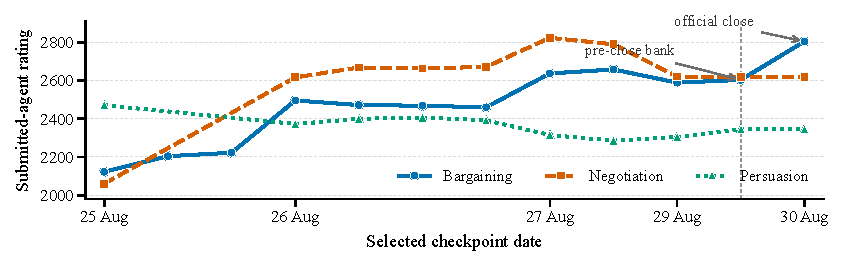
\includegraphics[width=0.96\linewidth]{figures/fig_strategy_evolution.pdf}
  \caption{Authenticated, irregularly spaced submitted-agent display
  snapshots. Lines connect observations only to make the rating reversals
  legible; they are not interpolated outcomes or an interrupted time-series
  estimate. The pre-close bank and official close are descriptive boundaries.}
  \label{fig:evolution}
\end{figure}

\subsection{From theory to retained behavior}

\begin{table}[h]
\centering
\small
\caption{Theory generated candidate actions; field evidence determined their
status. The final column describes the dated submitted configuration, not a
claim of equilibrium play.}
\label{tab:theory_evolution}
\begin{tabularx}{\linewidth}{@{}p{2.4cm}p{3.5cm}p{4.3cm}Y@{}}
\toprule
Family and benchmark & Candidate prediction & Observed failure or qualification & Retained behavior \\
\midrule
Bargaining: alternating offers and discounted continuation \citep{rubinstein1982} & Patience and horizon should determine acceptance and counteroffers; accepting $o\geq\delta c$ dominates one stipulated next-period accepted counter. & Later offer transforms could own the wire, and a later selected replay found accept-now worse than observed continuation in 45/45 joined histories under the P2 owner. The theorem never dominated arbitrary continuation. & Generic finite or reconstructed-hidden-cap recursion plus empirical floors, with one silent P2/H12/$\delta=.95$ owner. Broad guard off. \\
Negotiation: gains from trade, private information, and concession functions \citep{chatterjee1983incomplete,faratin1998negotiation} & Use visible ZOPA, infer safe reservation bounds, concede over time, and test leader-like anchors. & Two early diagnostics disfavored exponent 1.2, but later audits invalidated the measurement and left its sign unresolved. The randomized leader clone raised no-deals and failed its frozen checkpoint. & First-principles precedence and support-bounded terminal inference, followed by explicitly labeled empirical fallbacks. \\
Persuasion: committed obedience and repeated credibility \citep{kamenica2011bayesian,sobel1985credibility} & Recommend low items only within the one-shot obedience budget; richer language might preserve conversion. & GLEE has repeated, noncommitted messages. A fixed-history shadow selected 668 LOW all-push turns after three passed positives; 664 resolved and eight sold. An archived wording comparison lacked the denominator and provenance needed for an effect claim. & Deterministic tokens, pushing when prior expected value weakly cleared price, truth in other known-value cells, an adaptive unknown-value cutoff, the tight credibility reset, and one final V1 BUY-to-PASS safety veto. \\
\bottomrule
\end{tabularx}
\end{table}

\subsection{Dated submitted-agent rating chronology}

\begin{table}[h]
\centering
\small
\caption{Authenticated submitted-agent display movements around selected boundaries.
Every row is descriptive chronology. Family letters are B/N/P.}
\label{tab:rating_chronology}
\begin{tabularx}{\linewidth}{@{}p{2.25cm}p{3.25cm}p{4.4cm}Y@{}}
\toprule
Boundary & Strategy or operation & Display movement and games & Interpretation \\
\midrule
Aug. 25, 04:07--07:29 & High-share guard, whole negotiation V1, and narrow fixed P2 policy assembled at separate boundaries. & Overall $2220.76\rightarrow2467.17$ ($+246.41$) while ordinary play and several components changed. & History of the assembled stack, not attribution to any one component. \\
Aug. 26, 09:43--10:43 & Same 78-key overlay before and after a clean restart. & Overall $2495.16\rightarrow2513.66$; B $-23.98/133$, N $+51.84/133$, P $+27.63/134$. & One fixed stack produced sharply different family signs. \\
Aug. 27, 16:45--18:49 & Locked policy; family topology narrowed only to satisfy activity quotas. & All 79 assignments terminal: B $+21.03/20$, N $-33.78/22$, P $-29.42/37$; mean approximately $-14.06$. & Operational maintenance cost retained without selecting the winning family. \\
Aug. 29, 10:57--18:18 & Tight credibility reset copied into the final stack, followed by minimum-game close. & B $+14.60/19$, N $-1.02/19$, P $+40.12/25$; family mean $2505.09\rightarrow2522.99$. & The reset experiment had not met its own final rule, so the persuasion rise is not its effect. \\
Pre-close bank & Deterministic wrapper, LLM off, no active process. & B $2603.81/15{,}487$, N $2620.36/15{,}415$, P $2344.79/15{,}481$. & Valid dated checkpoint, not the final competition endpoint. \\
Aug. 30, 11:08--close & Same recorded overlay; bargaining, then bargaining and persuasion. & B $+201.01/152$; P $+.08/29$ rated plus one timeout; mean $2522.99\rightarrow2590.02$. & Complete exposure census, but unrandomized and without a full process-to-commit receipt. \\
Official close & Competition stopped accepting games at 11:59:59 UTC. & B $2804.82/15{,}639$, N $2620.36/15{,}415$, P $2344.87/15{,}510$. & Participant account second in the agent track and third on the combined board. \\
\bottomrule
\end{tabularx}
\end{table}

The checked-in source data for Figure~\ref{fig:evolution} record every plotted
timestamp, value, and ledger provenance. The largest trajectory lesson is not
the net rise. The same or near-identical policy eras produced both gains and
losses. For example, one unchanged development-profile bargaining stack moved from fitted
same-cell percentile $.5668$ ($n=471$) to $.5038$ ($n=498$), although
agreement remained 99.6\%. A deterministic leader-replica development profile moved
$+47.62$, then $-65.56$ in a fully joined 155-game shift, then $+31.43$ in a
fully joined 132-game shift. The last two fitted percentiles were $.49710$ and
$.49568$, with intervals spanning $.5$. Display movement should therefore
never be divided by game count and called a treatment effect.

\subsection{Competitors as hypothesis sources}

We distinguish five levels throughout. A \emph{participant account} is the
single entrant identity ranked by its best agent profile. An \emph{agent
profile} is one of at most five rated API agents under that account. An
\emph{execution slot} is our local runner and log label for a profile in one
era, not an account or strategy. The \emph{machine host} is the single computer
that ran those slots. An \emph{opponent profile label} is the name or type
exposed in about half of turn payloads; no opponent-account identifier was
exposed.

Competitor identities are anonymized as stable labels because opponent names
were disclosed in only about half the games and the shared pool may include
humans. Official documentation says in-account profiles are not paired, yet
some local opponent labels matched our execution-slot labels. Without an
opponent-account identifier, these records could reflect same-account play, a
nonunique display-name collision, or collector mislabeling, so we call them
identity-ambiguous rather than confirmed self-play. Named matches were excluded
where documented; hidden identities remain unclassifiable. The behavior summaries use
all directly observed games in their declared slices, not completed deals only.

\begin{table}[h]
\centering
\small
\caption{Direct competitor observations and the experiments they motivated.}
\label{tab:competitors}
\begin{tabularx}{\linewidth}{@{}p{2.65cm}p{4.35cm}Y@{}}
\toprule
Population & Direct observation & Evidential status \\
\midrule
Three then-leading public negotiation profiles A--C & 154 direct games. In hidden multi-round play, seller first-offer medians were $1.485$--$1.490B$ across 30 openings; buyer medians were $.8075$--$.8108B$ across 30 openings. Snapshot ratings ranged from 2649.25 to 2918.75. & Shared extreme-opening pattern across seats and horizons; no estimate of why the profiles rated highly. \\
Type-identified slice of A & Two completed cap-10 buyer games identify value $1.2B$ and midpoint normalized shares $.679,.679,.684,.717,.840$. & Direct only for one opponent profile and revealed type. Scaling to $1.0B$ or $1.5B$ was part of the randomized treatment, not a leader fact. \\
Four-source-profile clone evaluated on four in-account profiles & At a stopped 91-game read after an earlier $n=45$ look, candidate $+1.116$ rating/game ($n=44$) versus control $+.247$ ($n=47$), difference $+.869$. A new fixed-$z$ recomputation from the deidentified table gives normal interval $[-.73,2.47]$; the archived Welch interval was $[-.78,2.52]$. Profile-stratum-standardized difference was $+.991$, normal interval $[-.63,2.61]$. Candidate no-deals were 6.14 percentage points higher, Wald interval $[-12.0,24.3]$ percentage points, and one profile stratum was negative. & Game-hash randomized ITT under the stated assignment and interference assumptions. Repeated looks make intervals descriptive. Failed the precommitted promotion rule and was stopped. \\
Profiled bargaining opponents & Thirty-three profiles over 4,779 games had fitted acceptance thresholds from $.168$ to $.679$. & Real heterogeneity, but the opponent-specific exploit measured $-.0043$ diagnostic percentile and was removed. \\
\bottomrule
\end{tabularx}
\end{table}

The clone arm assigned the low bit of
$\operatorname{SHA256}(\texttt{nego\_top\_buyer\_clone\_v1}\,\|\,\texttt{game\_id})$
to candidate, with agent profile predeclared as a stratum before pooled analysis. The
deidentified companion table retains the assigned arm but withholds game IDs, so it
reproduces estimates without independently re-deriving assignment.

\section{Selected evidence ledger}
\label{app:ledger}

This ledger includes findings cited in the main paper, negative or invalid
studies that changed the final interpretation, and qualified signals needed to
explain the dated configuration. It is not a census of every exploratory plot
or threshold tried. The private machine-readable experiment and findings
ledgers remain the authoritative historical registry; that restriction creates
reporting-selection and reproducibility risk.

We could reconstruct a bounded registry cohort through the August 29 bank by
collapsing duplicate status updates and deployment epochs while retaining
separately enrolled replications. This is a census of named records in
\path{.ai/EXPERIMENTS.md}, not of the full exploratory universe. Handoff-only
candidates and threshold sweeps are excluded.

\begin{table}[h]
\centering
\small
\caption{Bounded named-record flow through the August 29 bank. Stage
rows overlap; the final three disposition rows partition all 35 records.}
\label{tab:registry_flow}
\begin{tabular}{@{}lr@{}}
\toprule
Registry-flow item & $n$ \\
\midrule
Named candidate or cohort records & 35 \\
Clearly implemented with documented action-changing reach & 33 \\
Code-loaded and armed live & 25 \\
Staged only & 1 \\
Passed a precommitted efficacy-promotion rule & 0 \\
Explicit adverse disposition & 7 \\
Stopped or superseded without an efficacy verdict & 17 \\
No terminal efficacy disposition & 11 \\
\bottomrule
\end{tabular}
\end{table}

The disposition counts do not estimate the prevalence of successful or failed
ideas. Six records were live or retained without promotion, three were built but
unrun, one was not built, and one was historical or unclear. A broader historical
universe would need a normalized registry with stable candidate identifiers.
The private source crosswalk in
\path{paper/data/experiment_registry_crosswalk.csv} freezes those 35 identifiers,
source ranges, inclusion categories, reach and live indicators, and dispositions.
Its normalization rules collapse deployment updates but retain separately enrolled
replications; one named factorial remains one record despite an independently
assigned sub-arm. The camera-ready artifact will replace private ledger paths
with stable released source IDs and checksums of sanitized evidence excerpts or
derived records.

\subsection{Structural and descriptive findings}

\begin{table}[h]
\centering
\small
\caption{Selected behavioral measurements used during development.}
\label{tab:full_findings}
\begin{tabularx}{\linewidth}{@{}p{3.4cm}p{4.0cm}Y@{}}
\toprule
Finding & Evidence & Interpretation \\
\midrule
Negotiation feasibility & Reconstructed generator: complete 6/6; hidden 6/16 value pairs under its independent-uniform model. & Both counts are conditional on the reconstructed support; hidden frequency and the 10/22 aggregate also require the stated joint and weighting assumptions. \\
Negotiation close rate & Complete 91.8\% ($n=805$); hidden 29.6\% ($n=2{,}295$). & Complete closure was 91.8\%; hidden closure was 78.9\% relative to the modeled feasible mass. Irrational trades mean the latter is not a literal ceiling. \\
Profitable incoming offers in later no-deals & 89 of 14,732 dependent decision turns, 0.6\%. & Turn-level selected evidence only; no unique-game rate is inferred. \\
Complete-information support & An archived check reported 911/911 outcomes consistent with the reconstructed value support. & Supports use of exact visible ZOPA, not hidden-type inference. \\
Bargaining role asymmetry & Historical local diagnostic over 4,001 games: Alice 71.5th percentile, Bob 28.8th. & Motivated role-specific diagnosis. These are not official role percentiles; later improvement is observational. \\
One-round response bracket & 384/384 below 0.90 span closed; 0/78 at or above 1.05 closed. & Descriptive bracket with an unobserved gap. \\
Persuasion wording & An archived comparison favored deterministic templates over LLM copy. & The frozen summary lacks the denominator, model and prompt provenance, and uncertainty needed for an effect claim. \\
Cross-stack dispersion & Endpoints described as identical spanned roughly 250 persuasion rating points over ten hours. & Commit and exposure provenance were incomplete; this is an observed range, not a statistical noise floor. \\
\bottomrule
\end{tabularx}
\end{table}

\subsection{Rejected, negative, and invalid studies}

\begin{table}[h]
\centering
\small
\caption{Hypotheses that were not allowed to become final-policy claims.}
\label{tab:negative}
\begin{tabularx}{\linewidth}{@{}p{3.0cm}p{4.9cm}Y@{}}
\toprule
Candidate & Result or defect & Verdict \\
\midrule
Aggressive visible-surplus share & Replay suggested $+0.0121$ percentile, but the clone auto-accepted unseen asks, used coarse bins, learned from selected agreements, and bundled three semantics. & Entire result invalidated. \\
Accept every profitable hidden offer & A biased selected replay covered 352 cases and reported $+0.07138$ without realized continuation. An archived corrected replay covered 375 exposed decisions, retained realized continuation, and reversed the sign. Its derived rows and resampling recipe were not preserved in the review artifact. & Unreproduced retrospective diagnostic with different estimands and denominators; removed before deployment, not ITT. \\
Ultimatum share 0.90/0.95 & Percentile changes $-0.003$ and about $-0.012$ to $-0.015$; close rate fell 1.6--2.0 points. & Rejected. \\
Faster concession & Two early diagnostics reported $-0.0166$ and $-0.0182$ local percentile for exponent 1.2 versus 2.0, but later audits invalidated the measurement and holdouts disagreed on direction. & Sign unresolved; retaining 2.0 was an operational choice, not an established effect. \\
Broad bargaining observed-gain rule & Three seeds $-0.0012,-0.0013,-0.0006$. & Rejected. \\
High-share bargaining override & Earlier selected replay found 35/35 favorable joined continuations and a positive adverse-missing bound. Under the later current P2 stack, accepting was worse than observed continuation in 45/45 joined cases, mean $-21.47$ pot points. & Stack-dependent retrospective reversal; configured child unreachable and no revival. \\
Unguarded stonewall release & Displayed rating moved about $-200$ over five uncontrolled hours. & Temporal co-movement motivated rollback; not an effect estimate. \\
Per-opponent exploitation & $-0.0043$ diagnostic percentile. & Removed. \\
Response-model offer engine & Sign changed across two continuation fits; unplayed asks lacked support. & Not identified. \\
Leader-trajectory clone & Early $+1.812$ rating/game at $n=45$ became $+0.869$ at a stopped $n=91$ read, nominal normal interval $[-0.73,2.47]$, with no-deals up 6.14 percentage points and one negative profile stratum. & Failed frozen promotion gates. \\
Negotiation score-floor counter & Historical hotfix closed 23/28 games with diagnostic percentile $.58208$; the later live floor closed 7/27 with $.20764$. & Era-confounded historical control, but rollback-grade safety failure; final flag explicit zero. \\
Cold-final reader & A stopped collector reported 11,737 outstanding records; a reader assigned low-rank outcomes to sufficiently old cold omissions. A later audit showed that 11,737 was not a reliable fleet total. & Reader corrected to retain cold omissions as unresolved; affected analyses reopened. \\
\bottomrule
\end{tabularx}
\end{table}

\subsection{Qualified positive signals}

The strongest pathwise reached-decision result is the $\delta<1$ bargaining
comparison reported above. It remained retrospective and the guard was off at
the bank. A complete-information unknown-horizon dynamic-stop audit found
21 retrospective triggers among 389 feasible buyer games: 14 better, 6 worse,
and 1 tie, with cohort-average diagnostic contrast $+0.01532$ and nominal
game-bootstrap interval $[0.00478,0.02725]$. The $.50$ rule came from an
observed threshold-grid break, so the interval does not cover selection. The
live deployment was not randomized; the draft does not call it causal. This was
a development-profile experiment, not a component of the submitted bank.

A fixed-history shadow of the positive-pass predicate selected 668 LOW all-push
turns on the submitted agent; 664 had observed outcomes, eight sold, and four remained
unresolved. Another stack's shadow selected 359 resolved turns and three sales.
The dependent, predicate-selected turns localized a behavior state and motivated
a prospective experiment. They were not submitted-agent interventions or policy-promotion
results.

\section{Expanded Agent Behavior Analysis}
\label{app:behavior}

\subsection{Audited action path}

The intended execution contract was:
\begin{enumerate}
  \item Route the visible game state to one family solver.
  \item Normalize the fields that family uses and compute a numerical plan.
  \item Apply ordered default-off gates, recording available trace events.
  \item Coerce the candidate into the exact server schema.
  \item Apply family postconditions and a legal fallback on error.
  \item Attempt to log the visible game state, plan, optional gate list, coarse source, and
  post-coercion action returned to the SDK.
\end{enumerate}
The returned action, not an intermediate variable, is the local behavioral
unit. This
prevents a policy from being called treated when a sanitizer later restores the
control action. It is not a server acknowledgement. Equality with official
history was established only for successfully joined subsets.

\subsection{Archive coverage and final-profile exposure}

The rules rank each participant account only by its best active profile
\citep{gleecompetition2026}. Placement is therefore account-level, while the
reported ratings and game counts belong to the focal profile that supplied the
maximum at close, not an ex ante held-out agent. Table~\ref{tab:archive_coverage}
inventories the focal profile and four historical development profiles used in
the paper's analyses; it is not a census of every profile identity ever
activated. Development profiles enter only explicitly labeled pooled audits.

\begin{table}[h]
\centering
\small
\caption{Local execution-slot/profile archive within one participant account.
``Final'' means a canonical joined terminal record, including the close-window
timeout. Only the focal row supports the 99.44\% public-total comparison; Development A was not
reconciled to a current public row.}
\label{tab:archive_coverage}
\begin{tabular}{@{}lrrrr@{}}
\toprule
Profile & Per-game records & Finals & Unresolved & Public total \\
\midrule
Submitted & 46,316 & 46,301 & 15 & 46,564 \\
Development A & 76,818 & 76,807 & 11 & not reconciled \\
Development B & 77,235 & 77,222 & 13 & 77,495 \\
Development C & 83,293 & 83,280 & 13 & 83,479 \\
Development D & 48,991 & 48,983 & 8 & 56,577 \\
\bottomrule
\end{tabular}
\end{table}

The submitted archive therefore contains canonical terminal joins for 99.44\%
of its 46,564 public rated games. Its flat result stream contains only 24,803
unique IDs, so
raw rows from that stream are never used as a denominator. The public game
endpoint is authenticated and does not expose histories to nonparticipants;
the remaining private records cannot be recovered by web scraping. Public
aggregate counts and ratings are therefore authoritative for lifetime totals.

Two narrower exposure windows are complete. The pre-close window ran from the
first fresh turn at 2026-08-29 05:27:36.596627 UTC through the last own action
at 12:48:08.480754 UTC, before a zero-active bank. The closing window ran from
2026-08-30 11:08:31.586 UTC through 11:59:57.872 UTC. Both used the same
recorded 81-key overlay and LLM-off wrapper; relevant tracked bargaining,
persuasion, and shared policy source was byte-equivalent, but no complete
process-to-commit receipt exists. Together the windows contain 245 assigned
games, 244 public game-count increments, one persuasion timeout, and 2,288 own
action records. Every assigned game has a canonical local join. All action
rows were tagged heuristic and logged zero local errors.

\begin{table}[h]
\centering
\small
\caption{Complete census of two final-profile exposure windows. Actions are
post-routing local records; totals describe behavior, not causal policy value.}
\label{tab:final_era_census}
\begin{tabularx}{\linewidth}{@{}p{2.2cm}p{3.2cm}p{4.2cm}Y@{}}
\toprule
Family & Games and role & Terminal outcomes & Recorded own actions \\
\midrule
Bargaining & 171; Alice/Bob $=89/82$ & 171 agreements & 503 offers, 414 rejects, 84 accepts \\
Negotiation & 19; seller/buyer $=10/9$ & 13 agreements, 3 walks, 3 no-deals & 10 initial offers, 171 rejects or counters, 7 accepts, 2 own walks; structural single-seller owner in 2 games and buyer/seller fallback router in 17 \\
Persuasion & 55; seller/buyer $=22/33$ & 54 completed, 1 timeout & Buyer yes/no $=456/201$; seller positive/negative $=316/124$. The pre-close subcohort contained 6 tight-reset turns in 2 games. \\
\bottomrule
\end{tabularx}
\end{table}

\begin{table}[h]
\centering
\small
\caption{Dated submitted-agent configuration, intended owner, and alignment boundary.}
\label{tab:alignment}
\begin{tabularx}{\linewidth}{@{}p{2.6cm}p{4.0cm}p{4.0cm}Y@{}}
\toprule
Component & Effective bank configuration & Intended owner and behavior & Evidence boundary \\
\midrule
Dispatcher & Family policy with LLM off; gate tracing configured. & Return a locally schema-coerced action, using a family fallback on exception. & Logging failure does not block return; traces are optional, incomplete, and not server acknowledgements. \\
Bargaining & Silent P2/H12/$\delta_2=.95$ owner on; broad discounted guard and its A/B arm off; high-share flag on but parent off. & Narrow P2 ladder and discounted floor own the exact silent cell; the generic planner owns the rest. & Public no-limit states use a reconstructed 99-round cap and a synthetic effective concession clock. The high-share child was unreachable, and the archive does not prove the loaded commit for every final process. \\
Negotiation & Submitted-agent default router V1 on. & First-principles owners take highest precedence, then an unflagged reservation-bound inference handles eligible hidden cap-10 buyer terminals; the observed-leader action function is buyer fallback. Seller fallback retains current decisions and an inherited message-only table in supported cells. & The inherited rules remained operational although the buyer rule's standalone experiment failed promotion gates; they are not causally validated. \\
Persuasion & Honest rounds 99, lie shading 0, buyer-v2, tight reset and V1 decline veto on, token templates. & Known values use all-push when prior expected value weakly clears price and otherwise low-item truth. Unknown values push while buy rate is absent or at least $.5$, then turn truthful. Posterior money gate precedes reset and veto. & In the complete pre-close subcohort, four text buyer games supplied 80 decisions; V1 missed and bought four repeated strict warnings in one game, and all revealed LOW. Decline-veto V2/V3 coverage was absent. \\
Analysis & Every enumerated A/B and probe flag in the archived overlay was explicit zero. & Recompute assignment, compare exact off/on returned actions, and join all terminal outcomes. & No complete final-PID manifest or bank-wide joined-action denominator exists, so universal conformance is not claimed. \\
\bottomrule
\end{tabularx}
\end{table}

\subsection{Forensic cases}

\paragraph{Parser abstention converted to purchase.}
For ``not recommended,'' the positive token was correctly suppressed by
negation, leaving zero phrase score. The parser returned abstention. The legacy
persuasion path then coerced every abstention to recommendation YES. The
alignment failure was therefore between tri-state parsing and binary fallback,
not inside token matching. This produced a positive recommendation signal, not
a direct purchase action. A strict decline guard was later constrained to
BUY-to-PASS changes, which makes its direction auditable but did not cover every
direct-warning phrase.

\paragraph{Treatment leakage.}
A negotiation surplus probe randomized a target before the offer branch. The
same target entered accept/reject variables, so treatment changed decisions on
turns that sent no offer. The outcome could estimate only the bundled policy,
not the intended response to a different ask. The probe was disabled.

\paragraph{Replay overlay mismatch.}
One candidate replay replaced the full control flag set instead of overlaying a
single key. A favorable comparison therefore measured two different stacks.
The corrected protocol freezes the base stack, changes one flag, and compares
the final submitted action byte for byte outside the scoped eligibility.

\paragraph{Non-firing gates.}
A flag nested under a parent omitted by the replay control produced a clean
$+0.0000$ null while never executing. The reachability contract now requires
positive eligible, fired, and changed-action counts before outcome analysis.

The result is limited but meaningful: case-level paired states changed as
predicted and selected successfully joined examples matched reconstructed
owners, while the audits exposed the mismatches above. The two exposure windows
have a complete process, local-action, and outcome denominator, but no lifetime
owner-to-wire conformance denominator is available. The configuration snapshot
alone does not establish that the reviewed commit produced every banked action.
Nor do these checks prove human-like
language understanding or economic optimality.

\section{Related work}
\label{app:related}

\paragraph{GLEE framework.}
Shapira et al. introduce a unified benchmark for two-player, sequential,
language-based bargaining, negotiation, and persuasion, parameterized by
horizon, information, communication, and family-specific market values
\citep{shapira2024glee}. Their evaluation compares self-gain, efficiency, and
fairness across agents and environments. We instead study the design, returned
behavior, and field outcome of one deterministic competition agent when
self-gain is transformed into a same-configuration, same-role percentile before
rating. The shared taxonomy is therefore our policy index, while the relative
score is the additional decision problem.

\paragraph{Rank objectives.}
GLEE's within-cell percentile resembles a rank-order incentive rather than a
standard expected-payoff objective \citep{lazear1981tournaments}. Under local
midranks it has a probability-of-superiority interpretation
\citep{mann1947test}, connecting it to pairwise ranking and U-statistic risk
\citep{clemencon2008ranking}. This should not be confused with $\alpha$-Rank,
which evaluates populations through evolutionary response graphs
\citep{omidshafiei2019alpharank}.

\paragraph{Bargaining and bilateral trade.}
The axiomatic Nash solution and strategic Rubinstein solution provide
complementary benchmarks
\citep{nash1950bargaining,rubinstein1982,binmore1986nash}. Two-sided private
information can create shading, delay, and inefficiency
\citep{chatterjee1983incomplete,chatterjee1987twosided,admati1987delay}, while
bilateral-trade mechanism constraints limit full efficiency
\citep{myerson1983bilateral}. Recent field evidence shows that incomplete-
information bargaining can still concentrate around simple splits
\citep{keniston2024splitting}. Among 192 selected completed
complete-information deals, median captured surplus was 49.4\%, although only
14\% lay in the 45--55\% band. Completion is selected, so this center does not
establish a field preference or an equilibrium.

\paragraph{Automated negotiation.}
Time-, resource-, and behavior-dependent concession functions
\citep{faratin1998negotiation}, incomplete-information agent strategies
\citep{fatima2002optimal}, and opponent modeling
\citep{jennings2001automated,baarslag2016opponent} motivate the agent's modular
policy. Negotiating-agent competitions have long revealed that heterogeneous
tactics and evaluation details matter \citep{baarslag2013anac}. Our additional
problem is that a payoff is converted to a cell-specific rank before rating.

\paragraph{Strategic communication and persuasion.}
Cheap-talk models study how preference conflict coarsens credible information
\citep{crawford1982strategic,farrell1996cheap}. Repetition can create credibility
\citep{sobel1985credibility}, while long communication can expand equilibrium
outcomes \citep{aumann2003long}. Bayesian persuasion instead grants
commitment to a signal structure \citep{kamenica2011bayesian}. GLEE combines
repetition, endogenous credibility, and parser-mediated language, closer to
recent long-run persuasion and language-based persuasion agents
\citep{best2024longrun,apel2022predicting,raifer2022automatic} than to any one
canonical model.

\paragraph{Language-model negotiation.}
Recent benchmarks study multi-issue negotiation, price bargaining, tactics,
and personality in LLM agents
\citep{abdelnabi2023negotiation,bianchi2024arena,xia2024bargaining}. GLEE
standardizes three economic families and a large configuration grid
\citep{shapira2024glee}. Both complete final-profile windows were configured
with LLM mode off, and all 2,288 local action records were tagged heuristic.
The contribution is not a new language model, but a theory-guided policy and an
audit method for the action returned at the agent interface.

\paragraph{Agent execution audits.}
Prior work already extends agent evaluation beyond terminal success through
intermediate progress and valid-action metrics, paired trace comparison,
structured runtime spans and fault injection, and trajectory failure
attribution
\citep{ma2024agentboard,zhou2026cta,seyedghorban2026observability,
zhang2025agentracer,chen2026trajectory}. Our contribution is narrower: a
GLEE-specific implementation-evidence contract that checks component
eligibility, gate firing, and exact post-coercion returned-action change before
joining economic outcomes. These checks detect unreachable gates, treatment
leakage, and downstream overwrites. They establish sampled execution alignment
and direct local action influence, not an effect on field outcomes; that still
requires pre-action randomization or controlled replay under explicit support,
consistency, and interference assumptions.

\paragraph{Empirical evaluation.}
Empirical game-theoretic analysis treats simulator or field interaction as a
way to estimate a reduced strategic game \citep{wellman2025egta}. Logged-policy
evaluation can be unbiased when action propensities and support are valid
\citep{li2011offline,dudik2014doubly}. These are support analogies for our
sequential setting; history-dependent off-policy evaluation needs stronger
trajectory assumptions \citep{jiang2016doubly}. Our negative results illustrate
their failure under selected deals, unplayed asks, adaptive opponents, and
stack mismatch. Precommitted looks follow the warning against
ordinary A/B peeking \citep{johari2017peeking}; formal continuous monitoring
would require adjusted sequential methods
\citep{pocock1977group,howard2021confidence}.

\section{Reproducibility, assets, and governance}
\label{app:reproducibility}
\label{app:governance}

The draft is tied to the official close at 2026-08-30 11:59:59 UTC. A stable
post-close public-board snapshot placed the participant account second in the
agent track and third on the combined human-and-agent board. The focal profile
displayed 2590.02 after 46,564 rated games, with bargaining
2804.82/15,639, negotiation 2620.36/15,415, and persuasion 2344.87/15,510.
The first-place agent-track profile displayed 2594.51, a 4.49-point gap. These
values are final competition outcomes for the adaptive account, not estimates
of component effects.

The archived pre-close row is retained to make the reversal auditable: at
2026-08-29 23:58:28 UTC, the same focal profile displayed 2522.99 after 46,383
games and the account provisionally led the agent track. The post-close row and
official endpoints are stored in
\path{paper/data/submitted_agent_leaderboard_snapshot.csv}. The submitted local
archive contains 46,301 canonical terminal joins, 99.44\% of the final public
total, plus the complete two-window exposure census in
Table~\ref{tab:final_era_census}.

The repository contains the deterministic family policies, runtime-flag
helpers, reachability checks, checked-in reconstructed-grid simulator, local percentile model,
tests, experiment ledger, and state snapshot. The general local CDF is a
diagnostic approximation: bargaining pools roles, both discount factors, and
message mode; negotiation omits opponent value and message state; and persuasion
omits some knowledge and scale dimensions. A separate negotiation seed helper
indexes the full value pair, role, horizon, information state, message mode, and
scale. It supports the hidden one-round seller's declared ex ante average in
Eq.~\eqref{eq:hidden_seller_seed_objective} and the narrow complete-information
score-floor diagnostic. Neither diagnostic should be described as the official
opponent-adjusted scorer.

The manifest below identifies the current source assets. The ordered 23-file
receipt in \path{paper/data/submitted_policy_asset_manifest.csv} records each
SHA-256; hashing its ordered \texttt{shasum -a 256} output gives
\texttt{1969fa1c5ef4c6d11d2ab565ece5fcbb40eb4e05a89fd7031edd58eaf521498c}.
The anonymous review bundle is deliberately separate from this private receipt.
It contains a standalone executable specification of effective behavior,
synthetic policy fixtures, deidentified aggregate tables, mathematical checks,
and figure and table generators. It excludes production source, deployment
switches, dormant arms, timestamps, game and profile identifiers, and any path
that can operate the live fleet. It can reproduce released arithmetic and
synthetic policy behavior, but cannot prove equivalence to withheld production
source or re-audit private joins and semantic labels.

Subject to licensing and the required data-governance determination, the
camera-ready release will additionally contain a frozen, sanitized policy
source snapshot, a non-operational effective-configuration specification, a
dependency lock, verification and analysis scripts, figure generators, and
deidentified tables. It will still exclude credentials, fleet controls, raw
logs and transcripts, game IDs, and opponent identities. Private provenance
ledgers will be represented by derived non-identifying aggregates rather than
redistributed verbatim.

\begin{table}[h]
\centering
\small
\caption{Policy-source artifact manifest. Paths are repository-relative.}
\label{tab:manifest}
\begin{tabularx}{\linewidth}{@{}p{4.1cm}Y@{}}
\toprule
Artifact & Purpose \\
\midrule
\path{glee_agent/config.py}, \path{runtime_flags.py}, \path{text.py}, \path{dispatch.py}, and \path{actions.py} & Runtime defaults, effective overlay, parsing, global precedence, schema repair, postguards, and fallback. All paths after the first share the \path{glee_agent/} prefix. \\
\path{glee_agent/strategies/bargaining.py} & Finite recursion, continuation, aspiration, and acceptance policy. \\
\path{glee_agent/bargaining_p2_commitment.py} & Banked silent P2/H12/$\delta_2=.95$ ladder and discounted acceptance floor. \\
\path{glee_agent/barg_offer.py} and \path{models/barg_bob_offer_v1.json} & Bob's fitted acceptance, local-rank, and refusal-continuation search. \\
\path{glee_agent/strategies/negotiation.py} & ZOPA, support, Boulware, hidden-value, and dynamic-stop policy. \\
\path{glee_agent/deterministic_negotiation.py}, \path{glee_agent/first_principles.py}, and \path{glee_agent/nego_hidden_terminal_inference.py} & Submitted-agent owner order, three designed structural cells, and ask-bounded hidden terminal buyer inference. \\
\path{glee_agent/top_buyer_clone.py}, \path{top_seller_message_clone.py}, \path{table_policy.py}, and \path{pricing.py} & Retained buyer paths, seller message overlay, table lookup, and pricing helpers. Paths after the first share the \path{glee_agent/} prefix. \\
\path{models/nego_policy_v1.json}, \path{negotiation_acceptance_v5.json}, \path{negotiation_value_posterior_v2.json}, and \path{stall_response_v1.json} & Active negotiation fitted thresholds, acceptance, value-posterior, and stall-response artifacts. Paths after the first share the \path{models/} prefix. \\
\path{glee_agent/strategies/persuasion.py} & Seller schedule, buyer posterior, parser gates, and credibility state. \\
\path{models/pers_buyer_prior_v1.json} & Fitted six-state persuasion-buyer prior weights. \\
\bottomrule
\end{tabularx}
\end{table}

\begin{table}[h]
\centering
\small
\caption{Evidence and reproduction manifest. Private ledgers are inputs to
derived release tables, not promised public files.}
\label{tab:evidence_manifest}
\begin{tabularx}{\linewidth}{@{}p{4.1cm}Y@{}}
\toprule
Artifact & Purpose \\
\midrule
\path{scripts/check_reachability.py} & Eligible, fired, and final-action-change checks. \\
\path{sim/percentile.py} & Local midrank diagnostic scorer. \\
\path{.ai/FINDINGS.md} & Frozen measured facts, including negative results. \\
\path{.ai/EXPERIMENTS.md} & Precommitted rules, cohorts, boundaries, and verdicts. \\
\path{paper/data/submitted_agent_rating_checkpoints.csv} & Authenticated rating checkpoints and line-level ledger provenance used by Figure~\ref{fig:evolution}. \\
\path{paper/data/submitted_agent_leaderboard_snapshot.csv} & Pre-close and official post-close ratings, game counts, account ranks, and source endpoints. \\
\path{paper/data/log_archive_coverage.csv} & Deidentified five-row historical archive inventory; only its focal row supports the 99.44\% lifetime-coverage boundary. \\
\path{paper/data/final_policy_era_census.csv} & Deidentified family, role, outcome, and action totals for the complete 63-game pre-close subcohort. \\
\path{paper/data/final_policy_two_window_census.csv} & Window, family, role, outcome, action, timeout, and error totals for all 245 final-profile assignments. \\
\path{paper/data/persuasion_parser_coverage.csv} & Frozen historical, complete post-V1, and pre-close parser denominators, counterexample counts, outcome joins, and canonical row hashes. \\
\path{paper/data/submitted_agent_bank_manifest.csv} & Frozen source commit, configuration hashes, pre-close boundaries, 81 recorded overlay flags, and behavior-affecting defaults absent from that overlay. \\
\path{paper/data/submitted_policy_asset_manifest.csv} & Ordered paths and individual SHA-256 values for the 23-file policy and fitted-model receipt. \\
\path{paper/data/clone_checkpoint_deidentified.csv} & Deidentified 91-game arm, profile-stratum, rating-change, and terminal-outcome table for the buyer-clone read. \\
\path{paper/data/experiment_registry_crosswalk.csv} & Private source crosswalk for the stable 35-record denominator; the public artifact will ship a derived registry with released source IDs and checksums. \\
\path{paper/analysis/analyze_clone_checkpoint.py} & Reproduces pooled, profile-stratum-standardized, and no-deal estimates and their stated normal intervals. \\
\path{paper/analysis/analyze_persuasion_parser_coverage.py} & Streams an authorized private turn archive to reproduce parser labels, complete denominators, purchased-outcome joins, and canonical row hashes. \\
\path{paper/analysis/verify_theory_code.py} & Checks exact rank identities, bargaining-CDF coarsening, the pooled hidden-seller seed argmax, and selected banked branches against the implementation. \\
\path{paper/analysis/verify_derived_tables.py} & Checks archive coverage and both pre-close and two-window game, action, timeout, and error totals. \\
\path{paper/analysis/verify_artifact_manifest.py} & Checks all 23 source/model hashes, their ordered checksum, the 81 overlay flags, and recorded runtime defaults. \\
\path{paper/review_artifact/verify_all.py} & Entry point for the isolated anonymous bundle: closed allowlist, checksum and privacy scans, synthetic policy and mathematical checks, released aggregate tables, and safe figure regeneration. \\
\path{paper/review/theory_code_audit.md} & Claim ledger separating proofs, implementation facts, empirical provenance, corrections, and unresolved limits. \\
\path{paper/figures/gen_fig_strategy_evolution.py} & Reproduces the descriptive rating chronology in Figure~\ref{fig:evolution}. \\
\path{paper/figures/gen_fig_rank_objective.py} & Reproduces Figure~\ref{fig:rank}. \\
\bottomrule
\end{tabularx}
\end{table}

The deidentified clone table removes game IDs, opponent names, values, prices,
messages, and timestamps. It reproduces the reported outcome summaries but
cannot re-audit hash assignment or source-to-wire joins. At the earlier read,
14 of 36 newly added rows failed the strict live-turn join and were retained
only after a deterministic match on execution slot, dashboard minute, public setup,
incoming price, returned action, and arm source. Their inclusion reduced the
apparent lift from $+2.51$ to $+1.81$ rating/game. Rating and payoff were not
join keys.

The archive does not contain a complete manifest linking every final process
ID to its loaded commit, start boundary, effective overlay hash, and joined
server-action coverage. The working remote remains private until the sanitized
camera-ready release. That artifact will reproduce the reported calculations,
figures, and deterministic policy checks, but cannot replay private live
interactions or re-audit every source-to-server join. At the draft freeze, the competition and
development profiles ran on one 10-core Apple M4 MacBook Air with 24 GB memory, running
macOS 26.5.1 on arm64 and Python 3.11.15. The two audited windows ran with LLM
mode off, trained no neural or language model for the submitted policy, and used
no GPU inference. They did use checked-in fitted empirical tables. An earlier development
comparison did use LLM-generated persuasion wording, but its provider, model
version, prompt procedure, and output-selection record were not preserved.
Historical per-analysis
wall time, peak memory, and total preliminary CPU use have not been
reconstructed, so this is not a complete compute account.

The authors did not recruit or instruct human participants. The official shared
pool can, however, contain human opponents. The draft makes no individual-level
human claim and withholds transcripts, but the authors should obtain an
institutional or organizer determination about whether analysis of those
interactions is exempt before submission. Organizer attestation is also needed
to bind the five public profile identifiers to the participant account, confirm
which profile supplied the account maximum, and resolve whether no-self-play
and display-name uniqueness explain the identity-ambiguous records. Strategic persuasion and bargaining
policies also have clear dual-use potential. The released strategic policy will
be framed for controlled benchmark use and will not authorize external
deployment without stronger safeguards and human-centered evaluation.

\fi

\ifpaperchecklist
\clearpage
\section*{NeurIPS Paper Checklist}

\begin{enumerate}

\item {\bf Claims}
    \item[] Question: Do the main claims made in the abstract and introduction accurately reflect the paper's contributions and scope?
    \item[] Answer: \answerYes{}
    \item[] Justification: The abstract and Sections~\ref{sec:introduction}--\ref{sec:competition} state the contribution as a rank-aware case study and returned-action audit, and distinguish identities, live descriptions, simulations, retrospective diagnostics, and causal claims.
    \item[] Guidelines:
    \begin{itemize}
        \item The answer \answerNA{} means that the abstract and introduction do not include the claims made in the paper.
        \item The abstract and/or introduction should clearly state the claims made, including the contributions made in the paper and important assumptions and limitations. A \answerNo{} or \answerNA{} answer to this question will not be perceived well by the reviewers.
        \item The claims made should match theoretical and experimental results, and reflect how much the results can be expected to generalize to other settings.
        \item It is fine to include aspirational goals as motivation as long as it is clear that these goals are not attained by the paper.
    \end{itemize}

\item {\bf Limitations}
    \item[] Question: Does the paper discuss the limitations of the work performed by the authors?
    \item[] Answer: \answerYes{}
    \item[] Justification: Sections~\ref{sec:behavior} and~\ref{sec:competition} discuss incomplete execution provenance, adaptive account-profile selection, private data, limited causal identification, an unreproduced replay, dual-use risks, and competition-specific scope.
    \item[] Guidelines:
    \begin{itemize}
        \item The answer \answerNA{} means that the paper has no limitation while the answer \answerNo{} means that the paper has limitations, but those are not discussed in the paper.
        \item The authors are encouraged to create a separate ``Limitations'' section in their paper.
        \item The paper should point out any strong assumptions and how robust the results are to violations of these assumptions (e.g., independence assumptions, noiseless settings, model well-specification, asymptotic approximations only holding locally). The authors should reflect on how these assumptions might be violated in practice and what the implications would be.
        \item The authors should reflect on the scope of the claims made, e.g., if the approach was only tested on a few datasets or with a few runs. In general, empirical results often depend on implicit assumptions, which should be articulated.
        \item The authors should reflect on the factors that influence the performance of the approach. For example, a facial recognition algorithm may perform poorly when image resolution is low or images are taken in low lighting. Or a speech-to-text system might not be used reliably to provide closed captions for online lectures because it fails to handle technical jargon.
        \item The authors should discuss the computational efficiency of the proposed algorithms and how they scale with dataset size.
        \item If applicable, the authors should discuss possible limitations of their approach to address problems of privacy and fairness.
        \item While the authors might fear that complete honesty about limitations might be used by reviewers as grounds for rejection, a worse outcome might be that reviewers discover limitations that aren't acknowledged in the paper. The authors should use their best judgment and recognize that individual actions in favor of transparency play an important role in developing norms that preserve the integrity of the community. Reviewers will be specifically instructed to not penalize honesty concerning limitations.
    \end{itemize}

\item {\bf Theory assumptions and proofs}
    \item[] Question: For each theoretical result, does the paper provide the full set of assumptions and a complete (and correct) proof?
    \item[] Answer: \answerYes{}
    \item[] Justification: Section~\ref{sec:introduction} states every condition for the one-step rating identity and derives the two-outcome terminal rank expression. Equation~\ref{eq:hidden-seller} is a declared finite construction, and Section~\ref{sec:strategy} labels the remaining game-theoretic rules as benchmarks or heuristics rather than theorems.
    \item[] Guidelines:
    \begin{itemize}
        \item The answer \answerNA{} means that the paper does not include theoretical results.
        \item All the theorems, formulas, and proofs in the paper should be numbered and cross-referenced.
        \item All assumptions should be clearly stated or referenced in the statement of any theorems.
        \item The proofs can either appear in the main paper or the supplemental material, but if they appear in the supplemental material, the authors are encouraged to provide a short proof sketch to provide intuition.
        \item Inversely, any informal proof provided in the core of the paper should be complemented by formal proofs provided in appendix or supplemental material.
        \item Theorems and Lemmas that the proof relies upon should be properly referenced.
    \end{itemize}

    \item {\bf Experimental result reproducibility}
    \item[] Question: Does the paper fully disclose all the information needed to reproduce the main experimental results of the paper to the extent that it affects the main claims and/or conclusions of the paper (regardless of whether the code and data are provided or not)?
    \item[] Answer: \answerNo{}
    \item[] Justification: Sections~\ref{sec:behavior} and~\ref{sec:competition} disclose denominators, evidence classes, and the main missing provenance. A prepared narrow bundle verifies selected arithmetic and synthetic policy fixtures, but it is not production-equivalent, is not yet available through an approved review channel, and cannot replay private interactions.
    \item[] Guidelines:
    \begin{itemize}
        \item The answer \answerNA{} means that the paper does not include experiments.
        \item If the paper includes experiments, a \answerNo{} answer to this question will not be perceived well by the reviewers: Making the paper reproducible is important, regardless of whether the code and data are provided or not.
        \item If the contribution is a dataset and\slash or model, the authors should describe the steps taken to make their results reproducible or verifiable.
        \item Depending on the contribution, reproducibility can be accomplished in various ways. For example, if the contribution is a novel architecture, describing the architecture fully might suffice, or if the contribution is a specific model and empirical evaluation, it may be necessary to either make it possible for others to replicate the model with the same dataset, or provide access to the model. In general. releasing code and data is often one good way to accomplish this, but reproducibility can also be provided via detailed instructions for how to replicate the results, access to a hosted model (e.g., in the case of a large language model), releasing of a model checkpoint, or other means that are appropriate to the research performed.
        \item While NeurIPS does not require releasing code, the conference does require all submissions to provide some reasonable avenue for reproducibility, which may depend on the nature of the contribution. For example
        \begin{enumerate}
            \item If the contribution is primarily a new algorithm, the paper should make it clear how to reproduce that algorithm.
            \item If the contribution is primarily a new model architecture, the paper should describe the architecture clearly and fully.
            \item If the contribution is a new model (e.g., a large language model), then there should either be a way to access this model for reproducing the results or a way to reproduce the model (e.g., with an open-source dataset or instructions for how to construct the dataset).
            \item We recognize that reproducibility may be tricky in some cases, in which case authors are welcome to describe the particular way they provide for reproducibility. In the case of closed-source models, it may be that access to the model is limited in some way (e.g., to registered users), but it should be possible for other researchers to have some path to reproducing or verifying the results.
        \end{enumerate}
    \end{itemize}


\item {\bf Open access to data and code}
    \item[] Question: Does the paper provide open access to the data and code, with sufficient instructions to faithfully reproduce the main experimental results, as described in supplemental material?
    \item[] Answer: \answerNo{}
    \item[] Justification: The working repository and verification bundle are private at submission. A sanitized production-equivalent camera-ready release is planned but remains conditional on licensing, data-use permission, and privacy review; raw transcripts, identities, credentials, and operational controls will remain withheld.
    \item[] Guidelines:
    \begin{itemize}
        \item The answer \answerNA{} means that paper does not include experiments requiring code.
        \item Please see the NeurIPS code and data submission guidelines (\url{https://neurips.cc/public/guides/CodeSubmissionPolicy}) for more details.
        \item While we encourage the release of code and data, we understand that this might not be possible, so \answerNo{} is an acceptable answer. Papers cannot be rejected simply for not including code, unless this is central to the contribution (e.g., for a new open-source benchmark).
        \item The instructions should contain the exact command and environment needed to run to reproduce the results. See the NeurIPS code and data submission guidelines (\url{https://neurips.cc/public/guides/CodeSubmissionPolicy}) for more details.
        \item The authors should provide instructions on data access and preparation, including how to access the raw data, preprocessed data, intermediate data, and generated data, etc.
        \item The authors should provide scripts to reproduce all experimental results for the new proposed method and baselines. If only a subset of experiments are reproducible, they should state which ones are omitted from the script and why.
        \item At submission time, to preserve anonymity, the authors should release anonymized versions (if applicable).
        \item Providing as much information as possible in supplemental material (appended to the paper) is recommended, but including URLs to data and code is permitted.
    \end{itemize}


\item {\bf Experimental setting/details}
    \item[] Question: Does the paper specify all the training and test details (e.g., data splits, hyperparameters, how they were chosen, type of optimizer) necessary to understand the results?
    \item[] Answer: \answerNo{}
    \item[] Justification: Sections~\ref{sec:behavior}--\ref{sec:competition} report assignment units, cohorts, sample counts, and evidence status, but some historical seeds, resampling recipes, assignment details, and process-to-commit-to-server records were not preserved.
    \item[] Guidelines:
    \begin{itemize}
        \item The answer \answerNA{} means that the paper does not include experiments.
        \item The experimental setting should be presented in the core of the paper to a level of detail that is necessary to appreciate the results and make sense of them.
        \item The full details can be provided either with the code, in appendix, or as supplemental material.
    \end{itemize}

\item {\bf Experiment statistical significance}
    \item[] Question: Does the paper report error bars suitably and correctly defined or other appropriate information about the statistical significance of the experiments?
    \item[] Answer: \answerNo{}
    \item[] Justification: The clone interval is a nominal unadjusted normal interval after two looks, not a confirmatory confidence interval. The archived replay lacks a preserved resampling recipe, so the core reports only its unreproduced direction reversal.
    \item[] Guidelines:
    \begin{itemize}
        \item The answer \answerNA{} means that the paper does not include experiments.
        \item The authors should answer \answerYes{} if the results are accompanied by error bars, confidence intervals, or statistical significance tests, at least for the experiments that support the main claims of the paper.
        \item The factors of variability that the error bars are capturing should be clearly stated (for example, train/test split, initialization, random drawing of some parameter, or overall run with given experimental conditions).
        \item The method for calculating the error bars should be explained (closed form formula, call to a library function, bootstrap, etc.)
        \item The assumptions made should be given (e.g., Normally distributed errors).
        \item It should be clear whether the error bar is the standard deviation or the standard error of the mean.
        \item It is OK to report 1-sigma error bars, but one should state it. The authors should preferably report a 2-sigma error bar than state that they have a 96\% CI, if the hypothesis of Normality of errors is not verified.
        \item For asymmetric distributions, the authors should be careful not to show in tables or figures symmetric error bars that would yield results that are out of range (e.g., negative error rates).
        \item If error bars are reported in tables or plots, the authors should explain in the text how they were calculated and reference the corresponding figures or tables in the text.
    \end{itemize}

\item {\bf Experiments compute resources}
    \item[] Question: For each experiment, does the paper provide sufficient information on the computer resources (type of compute workers, memory, time of execution) needed to reproduce the experiments?
    \item[] Answer: \answerNo{}
    \item[] Justification: The submitted policy required no model training or inference-time LLM call, but this four-page report does not provide host, memory, per-analysis wall time, peak memory, or total exploratory CPU use for the competition period.
    \item[] Guidelines:
    \begin{itemize}
        \item The answer \answerNA{} means that the paper does not include experiments.
        \item The paper should indicate the type of compute workers CPU or GPU, internal cluster, or cloud provider, including relevant memory and storage.
        \item The paper should provide the amount of compute required for each of the individual experimental runs as well as estimate the total compute.
        \item The paper should disclose whether the full research project required more compute than the experiments reported in the paper (e.g., preliminary or failed experiments that didn't make it into the paper).
    \end{itemize}

\item {\bf Code of ethics}
    \item[] Question: Does the research conducted in the paper conform, in every respect, with the NeurIPS Code of Ethics \url{https://neurips.cc/public/EthicsGuidelines}?
    \item[] Answer: \answerNo{}
    \item[] Justification: The work withholds transcripts and reports no opponent identities or participant-level claims, but the shared pool may include humans and the required organizer or institutional determination has not yet been obtained. This draft must not be submitted until that review is resolved.
    \item[] Guidelines:
    \begin{itemize}
        \item The answer \answerNA{} means that the authors have not reviewed the NeurIPS Code of Ethics.
        \item If the authors answer \answerNo, they should explain the special circumstances that require a deviation from the Code of Ethics.
        \item The authors should make sure to preserve anonymity (e.g., if there is a special consideration due to laws or regulations in their jurisdiction).
    \end{itemize}


\item {\bf Broader impacts}
    \item[] Question: Does the paper discuss both potential positive societal impacts and negative societal impacts of the work performed?
    \item[] Answer: \answerYes{}
    \item[] Justification: Section~\ref{sec:competition} discusses the value of auditable strategic agents and names risks from manipulative persuasion, human-opponent exploitation, imitation, and transfer beyond the benchmark.
    \item[] Guidelines:
    \begin{itemize}
        \item The answer \answerNA{} means that there is no societal impact of the work performed.
        \item If the authors answer \answerNA{} or \answerNo, they should explain why their work has no societal impact or why the paper does not address societal impact.
        \item Examples of negative societal impacts include potential malicious or unintended uses (e.g., disinformation, generating fake profiles, surveillance), fairness considerations (e.g., deployment of technologies that could make decisions that unfairly impact specific groups), privacy considerations, and security considerations.
        \item The conference expects that many papers will be foundational research and not tied to particular applications, let alone deployments. However, if there is a direct path to any negative applications, the authors should point it out. For example, it is legitimate to point out that an improvement in the quality of generative models could be used to generate Deepfakes for disinformation. On the other hand, it is not needed to point out that a generic algorithm for optimizing neural networks could enable people to train models that generate Deepfakes faster.
        \item The authors should consider possible harms that could arise when the technology is being used as intended and functioning correctly, harms that could arise when the technology is being used as intended but gives incorrect results, and harms following from (intentional or unintentional) misuse of the technology.
        \item If there are negative societal impacts, the authors could also discuss possible mitigation strategies (e.g., gated release of models, providing defenses in addition to attacks, mechanisms for monitoring misuse, mechanisms to monitor how a system learns from feedback over time, improving the efficiency and accessibility of ML).
    \end{itemize}

\item {\bf Safeguards}
    \item[] Question: Does the paper describe safeguards that have been put in place for responsible release of data or models that have a high risk for misuse (e.g., pre-trained language models, image generators, or scraped datasets)?
    \item[] Answer: \answerNA{}
    \item[] Justification: The paper does not release a high-risk pretrained model or scraped dataset. Raw transcripts remain private because they may contain opponent-generated text.
    \item[] Guidelines:
    \begin{itemize}
        \item The answer \answerNA{} means that the paper poses no such risks.
        \item Released models that have a high risk for misuse or dual-use should be released with necessary safeguards to allow for controlled use of the model, for example by requiring that users adhere to usage guidelines or restrictions to access the model or implementing safety filters.
        \item Datasets that have been scraped from the Internet could pose safety risks. The authors should describe how they avoided releasing unsafe images.
        \item We recognize that providing effective safeguards is challenging, and many papers do not require this, but we encourage authors to take this into account and make a best faith effort.
    \end{itemize}

\item {\bf Licenses for existing assets}
    \item[] Question: Are the creators or original owners of assets (e.g., code, data, models), used in the paper, properly credited and are the license and terms of use explicitly mentioned and properly respected?
    \item[] Answer: \answerNo{}
    \item[] Justification: The GLEE platform and NeurIPS template are credited and linked, but a complete version and license inventory for all competition-side assets is not yet available in this draft.
    \item[] Guidelines:
    \begin{itemize}
        \item The answer \answerNA{} means that the paper does not use existing assets.
        \item The authors should cite the original paper that produced the code package or dataset.
        \item The authors should state which version of the asset is used and, if possible, include a URL.
        \item The name of the license (e.g., CC-BY 4.0) should be included for each asset.
        \item For scraped data from a particular source (e.g., website), the copyright and terms of service of that source should be provided.
        \item If assets are released, the license, copyright information, and terms of use in the package should be provided. For popular datasets, \url{paperswithcode.com/datasets} has curated licenses for some datasets. Their licensing guide can help determine the license of a dataset.
        \item For existing datasets that are re-packaged, both the original license and the license of the derived asset (if it has changed) should be provided.
        \item If this information is not available online, the authors are encouraged to reach out to the asset's creators.
    \end{itemize}

\item {\bf New assets}
    \item[] Question: Are new assets introduced in the paper well documented and is the documentation provided alongside the assets?
    \item[] Answer: \answerNA{}
    \item[] Justification: No new public dataset, model, or code asset is released with this draft. The planned camera-ready artifact will include licenses and a data-access statement.
    \item[] Guidelines:
    \begin{itemize}
        \item The answer \answerNA{} means that the paper does not release new assets.
        \item Researchers should communicate the details of the dataset\slash code\slash model as part of their submissions via structured templates. This includes details about training, license, limitations, etc.
        \item The paper should discuss whether and how consent was obtained from people whose asset is used.
        \item At submission time, remember to anonymize your assets (if applicable). You can either create an anonymized URL or include an anonymized zip file.
    \end{itemize}

\item {\bf Crowdsourcing and research with human subjects}
    \item[] Question: For crowdsourcing experiments and research with human subjects, does the paper include the full text of instructions given to participants and screenshots, if applicable, as well as details about compensation (if any)?
    \item[] Answer: \answerNo{}
    \item[] Justification: The authors did not recruit, instruct, or compensate participants, but the shared opponent pool may include humans. Organizer authorization and the applicable institutional classification for this secondary analysis remain unresolved.
    \item[] Guidelines:
    \begin{itemize}
        \item The answer \answerNA{} means that the paper does not involve crowdsourcing nor research with human subjects.
        \item Including this information in the supplemental material is fine, but if the main contribution of the paper involves human subjects, then as much detail as possible should be included in the main paper.
        \item According to the NeurIPS Code of Ethics, workers involved in data collection, curation, or other labor should be paid at least the minimum wage in the country of the data collector.
    \end{itemize}

\item {\bf Institutional review board (IRB) approvals or equivalent for research with human subjects}
    \item[] Question: Does the paper describe potential risks incurred by study participants, whether such risks were disclosed to the subjects, and whether Institutional Review Board (IRB) approvals (or an equivalent approval/review based on the requirements of your country or institution) were obtained?
    \item[] Answer: \answerNo{}
    \item[] Justification: No author-side institutional or exemption determination has yet been recorded. Because the shared pool may include humans, the authors must obtain the applicable determination and organizer confirmation before submission.
    \item[] Guidelines:
    \begin{itemize}
        \item The answer \answerNA{} means that the paper does not involve crowdsourcing nor research with human subjects.
        \item Depending on the country in which research is conducted, IRB approval (or equivalent) may be required for any human subjects research. If you obtained IRB approval, you should clearly state this in the paper.
        \item We recognize that the procedures for this may vary significantly between institutions and locations, and we expect authors to adhere to the NeurIPS Code of Ethics and the guidelines for their institution.
        \item For initial submissions, do not include any information that would break anonymity (if applicable), such as the institution conducting the review.
    \end{itemize}

\item {\bf Declaration of LLM usage}
    \item[] Question: Does the paper describe the usage of LLMs if it is an important, original, or non-standard component of the core methods in this research? Note that if the LLM is used only for writing, editing, or formatting purposes and does \emph{not} impact the core methodology, scientific rigor, or originality of the research, declaration is not required.
    %this research?
    \item[] Answer: \answerNo{}
    \item[] Justification: The submitted agent is deterministic and LLM-free, but development included an archived comparison involving LLM-generated persuasion wording. Its provider, model version, prompt procedure, and output-selection record were not preserved well enough for complete methodological disclosure.
    \item[] Guidelines:
    \begin{itemize}
        \item The answer \answerNA{} means that the core method development in this research does not involve LLMs as any important, original, or non-standard components.
        \item Please refer to our LLM policy in the NeurIPS handbook for what should or should not be described.
    \end{itemize}

\end{enumerate}

\fi

\end{document}
